\documentclass[12pt,a4paper]{article}

% -- Codificació i llenguatge
\usepackage[catalan]{babel}
\usepackage[T1]{fontenc}
\usepackage[utf8]{inputenc}

% -- Layout
\usepackage{geometry}
\usepackage[defaultlines=3,all]{nowidow}
\usepackage{setspace}
\usepackage{titlesec}

% -- Tipografia i símbols
\usepackage{amsmath}
\usepackage{amssymb}

% -- Grafics
\usepackage{graphicx}
\usepackage{tikz}
\usepackage{pgfgantt}

% -- Formatat i taules
\usepackage{adjustbox}
\usepackage{array}
\usepackage{booktabs}
\usepackage{enumitem}
\usepackage{float}
\usepackage{longtable}
\usepackage{pdflscape}
\usepackage{tabularx}
\usepackage{xcolor}

\usepackage[hidelinks]{hyperref}

\geometry{margin=2.5cm}
\setstretch{1.2}
\raggedbottom

\begin{document}

\begin{titlepage}
    \centering
    % -- LOGOTIPO O IMAGEN (OPCIONAL) --
    % Descomenta las siguientes líneas y reemplaza 'ruta/a/tu/logo.png' por la ruta de tu imagen.
    % \vspace*{1cm}
    % \includegraphics[width=0.4\textwidth]{ruta/a/tu/logo.png} 
    % \vspace{1.5cm}
    % -----------------------------------

    % -- TÍTULO DEL PROYECTO --
    % Uso de \textsf para una fuente sans-serif, más moderna para títulos.
    {\huge\textbf{Sistema de Votació Electrónica \\ basat en \textit{Blockchain}}\par}
    
    % -- LÍNEA DIVISORIA (OPCIONAL) --
    % \vspace{0.5cm}
    % \hrulefill
    % \vspace{0.5cm}
    % --------------------------------

    \vspace{2.5cm} % Espacio aumentado para separar del título

    % -- OBJETIVO DEL PROYECTO --
    \begin{center}
        \textbf{\large Objectiu del projecte}\\[0.5cm]
        % Usamos \parbox para limitar el ancho del texto y que se vea más centrado y limpio.
        \parbox{0.85\textwidth}{
            \centering
            Desenvolupament d'un sistema de votació electrònica descentralitzat,
            segur, transparent i auditable, amb finalitat formativa per a l'aprenentatge
            de la tecnologia \textit{blockchain} i els contractes intel·ligents.
        }
    \end{center}

    \vspace{3cm} % Espacio aumentado para separar del objetivo

    % -- EQUIPO DE DESARROLLO --
    \textbf{\large Equip de desenvolupament}\\[0.8cm]
    % Aumentamos el tamaño de la fuente para los nombres.
    {\large
        Jordi Vanyó \\
        Dylan Luigi \\
        Toni Contestí \\
        Marc Link
    }
    
    \vfill % Empuja la fecha hacia la parte inferior de la página

    % -- FECHA --
    % Aumentamos el tamaño y la ponemos en negrita.
    {\large \textbf{Maig 2026}}
    \vspace*{1cm} % Un pequeño margen inferior

\end{titlepage}

\tableofcontents
\newpage

\section{Motivació i problema a resoldre}

Actualment, els sistemes de votació tradicionals tenen un problema de fons evident: \textbf{ens obliguen a confiar cegament en una autoritat central}. 
Aquesta dependència d'una única entitat actua com a punt únic de fallada i, alhora, genera dubtes raonables sobre la transparència, la seguretat i la integritat de tot el procés electoral. 
Ens trobam davant de sistemes on hi ha un risc real de manipulació dels resultats o corrupció interna, on \textbf{els errors humans durant el recompte són freqüents}, i on \textbf{resulta pràcticament impossible que un ciutadà o una entitat externa auditi el procés de manera independent}.

D'altra banda, la simple digitalització d'aquest procés mitjançant aplicacions web o servidors convencionals està lluny de solucionar el problema de fons. De fet, el que fa és traslladar-lo a un altre escenari. 
Les solucions digitals centralitzades obrin la porta a nous \textbf{riscos de ciberseguretat}, com ara vulnerabilitats del codi, atacs informàtics o caigudes de servidors. 
A això cal sumar-hi la \textbf{desconfiança generalitzada de la població a l'hora de fer tràmits tan crítics per internet} i les \textbf{dificultats d'ús per a persones amb menys habilitats digitals}, la qual cosa suposa una barrera d'entrada important.

Davant d'aquest context, la nostra motivació principal és dissenyar i desenvolupar una alternativa real que elimini la necessitat de confiança cega: \textbf{un sistema de votació electrònica completament descentralitzat basat en tecnologia \hyperlink{def:blockchain}{\textit{blockchain}}}. 
\textbf{Volem crear un entorn on el problema de la confiança es resolgui directament pel propi disseny de l'arquitectura i del codi}. 
Aquest sistema ha de ser capaç de garantir una transparència verificable, permetent que qualsevol persona pugui comprovar el bon funcionament de la xarxa sense comprometre l'\hyperlink{def:anonimat}{anonimat} real del votant ni les dades sensibles \cite{su16114387} \cite{nakamoto} \cite{vladucu2023} \cite{berenjestanaki2024}.

La naturalesa de la \hyperlink{def:blockchain}{\textit{blockchain}} ens permet assegurar la integritat criptogràfica del sistema. Una vegada s'emet un vot, la xarxa el protegeix matemàticament i fa que sigui impossible de modificar o eliminar. 
A més, el disseny mateix de la xarxa evita l'existència de vots dobles i proporciona una \hyperlink{def:auditabilitat}{auditabilitat} independent, ja que podem \hyperlink{def:verificabilitat}{verificar} els resultats de forma totalment lliure i precisa sense haver de demanar permís a cap autoritat.

Finalment, més enllà de la utilitat i l'impacte d'aquesta solució tecnològica a la societat, aquest projecte neix d'una motivació acadèmica. Volem aprofitar aquest projecte per adquirir coneixements pràctics reals sobre el funcionament intern de la tecnologia \hyperlink{def:blockchain}{\textit{blockchain}}, aprendre a programar contractes intel·ligents (\hyperlink{def:smartcontract}{\textit{smart contracts}}) \cite{buterin} i entendre com es dissenyen i es despleguen \hyperlink{def:dapp}{aplicacions descentralitzades} segures.

\section{Objectius}

L'objectiu principal d'aquest projecte és el desenvolupament d'un prototip funcional d'un sistema de votació electrònica basat en tecnologia \hyperlink{def:blockchain}{\textit{blockchain}} que garanteixi seguretat, transparència i anonimat. Concretament, els objectius es divideixen entre els del sistema i formatius:

\subsubsection*{Objectius del sistema}
\begin{enumerate}
    \item \textbf{Autenticació segura i vot únic:} \\ Implementar un mecanisme robust d'autenticació que verifiqui la identitat de l'usuari i asseguri que cada elector només pugui emetre el seu vot una única vegada.
    \item \textbf{Privacitat i anonimat absoluts:} \\ Garantir que el vot de cada individu quedi desvinculat de la seva identitat real, protegint completament l'anonimat del procés.
    \item \textbf{Transparència i verificabilitat pública:} \\ Desenvolupar un sistema auditable on qualsevol ciutadà o auditor extern pugui verificar els resultats de l'elecció sense comprometre la privacitat dels votants.
    \item \textbf{Accessibilitat i usabilitat:} \\ Crear una interfície web intuïtiva que faciliti l'experiència d'usuari i elimini les barreres tecnològiques per als votants.
\end{enumerate}

\subsubsection*{Objectius formatius}
\begin{enumerate}
    \setcounter{enumi}{4}
    \item \textbf{Domini de la tecnologia \hyperlink{def:blockchain}{\textit{blockchain}}:} \\ Aprendre els fonaments pràctics i teòrics de les cadenes de blocs i comprendre l'arquitectura dels sistemes descentralitzats.
    \item \textbf{Implementació de \textit{smart contracts}:} \\ Comprendre i programar contractes intel·ligents capaços d'automatitzar i assegurar processos digitals de manera autònoma.
    \item \textbf{Exploració de nous casos d'ús descentralitzats:} \\ Validar el potencial de la tecnologia \hyperlink{def:blockchain}{\textit{blockchain}} en aplicacions reals més enllà de les criptomonedes, com ara la contractació digital, els sistemes distribuïts i la certificació de dades.
\end{enumerate}

\section{Abast del projecte}

\subsection{Requisits funcionals}

L'abast d'aquest projecte comprèn el disseny i desenvolupament d'un prototip funcional d'un sistema de votació electrònica descentralitzada utilitzant \hyperlink{def:blockchain}{\textit{blockchain}}.

\subsubsection{Connexió de la cartera digital i verificació del cens:}

Garanteix que només puguin votar les persones prèviament autoritzades al cens, eliminant la necessitat d'un servidor centralitzat i mantenint l'\hyperlink{def:anonimat}{anonimat}, ja que s'utilitzen \hyperlink{def:adreca}{adreces} criptogràfiques en lloc de dades personals.

En lloc d'un inici de sessió tradicional, l'aplicació web permetrà al votant autenticar-se connectant la seva cartera digital.
Un cop connectada, l'aplicació consultarà directament el \hyperlink{def:smartcontract}{contracte intel·ligent} (\textit{smart contract}) per verificar si l'\hyperlink{def:adreca}{adreça} pública de l'usuari està registrada a la llista d'admesos (cens electoral) i comprovarà que no ha emès ja el seu vot.

Elimina la dependència d'una autoritat central per a la verificació d'identitat. 
El votant obté una garantia matemàtica que el seu accés és legítim, mentre que l'organitzador delega la lògica de control al \hyperlink{def:smartcontract}{contracte intel·ligent}, reduint la gestió manual i el risc d'errors humans.

\paragraph{Criteris d'acceptació:}
\begin{enumerate}[label=\roman*.]
    \item El votant ha de poder connectar la seva \textit{wallet} a la interfície web de forma senzilla.
    \item El \textit{smart contract} ha de validar en temps real si l'adreça connectada pertany al cens autoritzat.
    \item Si l'usuari no està al cens o ja ha votat prèviament, la interfície ha de bloquejar l'accés a la papereta de vot i mostrar un missatge d'error clar.
\end{enumerate}

\subsubsection{Emissió i registre del vot (\textit{Smart Contract}):}
Permet a l'usuari seleccionar una opció i registrar el seu vot de manera inalterable a la \hyperlink{def:blockchain}{cadena de blocs} \cite{nakamoto}.

Garanteix que el vot no pugui ser modificat ni eliminat un cop emès. 
A més, proporciona al votant una experiència d'ús clara, accessible i amb retroalimentació visual immediata. La prevenció del doble vot es garanteix per disseny a nivell de \hyperlink{def:smartcontract}{contracte intel·ligent}, eliminant qualsevol possibilitat de manipulació per part d'intermediaris.

El sistema contempla dos tipus de vots diferenciats: els vots sobre propostes d'eleccions (mitjançant els quals els usuaris expressen el seu suport a la creació d'un nou procés electoral) i els vots sobre eleccions actives (on els usuaris trien entre les opcions disponibles dins d'un procés electoral ja generat). Ambdós tipus de vot segueixen el mateix mecanisme de registre immutable a la cadena de blocs.

\paragraph{Criteris d'acceptació:}
\begin{enumerate}[label=\roman*.]
    \item El votant ha de poder connectar la seva \hyperlink{def:wallet}{\textit{wallet}} a la interfície web de forma senzilla.
    \item El \hyperlink{def:smartcontract}{\textit{smart contract}} ha de validar en temps real si l'\hyperlink{def:adreca}{adreça} connectada pertany al cens autoritzat.
    \item Si l'usuari no està al cens o ja ha votat prèviament, la interfície ha de bloquejar l'accés a la papereta de vot i mostrar un missatge d'error clar.
    \item El sistema ha de distingir correctament entre vots a propostes d'eleccions i vots a eleccions actives, registrant cadascun al mecanisme d'emmagatzematge corresponent del contracte.
\end{enumerate}

\subsubsection{Proposta i generació d'eleccions:}

Mòdul integrat al contracte intel·ligent que permet als usuaris del cens proposar nous processos electorals de manera descentralitzada. Quan una proposta assoleix un llindar predefinit de vots favorables, el contracte genera automàticament l'elecció corresponent.

El cicle de vida d'un procés electoral segueix una seqüència determinista gestionada íntegrament pel contracte intel·ligent: un usuari del cens registra una proposta d'elecció, els membres del cens voten a favor o en contra d'aquesta proposta, i si es compleix el llindar establert, el contracte genera l'elecció amb les dates i opcions definides a la proposta original. Un cop generada, l'elecció passa a estar disponible perquè els votants emetin el seu vot.

Aquesta mecànica elimina la necessitat d'un administrador central que decideixi quines eleccions es convoquen. La decisió de crear un procés electoral és col·lectiva i queda registrada de forma transparent i auditable a la cadena de blocs.

\paragraph{Criteris d'acceptació:}
\begin{enumerate}[label=\roman*.]
    \item Qualsevol usuari del cens ha de poder registrar una proposta d'elecció mitjançant una transacció signada.
    \item El contracte ha de rebutjar propostes duplicades i limitar el registre a una única proposta per adreça per a un mateix tema.
    \item Els membres del cens han de poder votar a favor d'una proposta, i el contracte ha de registrar aquests vots evitant-ne la duplicació.
    \item Quan una proposta assoleix el llindar de vots establert, el contracte ha de generar automàticament l'elecció corresponent sense intervenció externa.
\end{enumerate}

\subsubsection{Recompte automàtic i escrutini públic:}
Unificació del procés d'emmagatzematge i recompte de vots directament a la \textit{blockchain}, permetent la lectura transparent dels resultats.

Els vots processats s'emmagatzemen com a transaccions immutables. El contracte actualitza l'estat del recompte de manera autònoma i transparent per a cada vot vàlid. 
S'elimina la necessitat d'una junta electoral per comptar paperetes, oferint als auditors la capacitat de verificar la integritat dels resultats directament sobre la cadena de blocs sense demanar permís.

\paragraph{Criteris d'acceptació:}
\begin{enumerate}[label=\roman*.]
    \item L'estat del recompte s'ha d'actualitzar automàticament via contracte intel·ligent per a cada vot vàlid rebut i no pot ser modificat manualment.
    \item La interfície web ha de consultar i mostrar els resultats directament des de la xarxa \textit{blockchain}, sense bases de dades intermèdies.
    \item Per garantir que l'escrutini no influeixi en la intenció de vot, els resultats acumulats només seran accessibles (o desencriptats) un cop el contracte intel·ligent marqui l'elecció com a ``Tancada''.
\end{enumerate}

\subsubsection{Verificabilitat individual del votant:}
Capacitat del sistema per permetre a l'elector comprovar de manera independent que el seu vot ha estat processat i inclòs en el recompte final.

En els sistemes tradicionals, un cop el vot entra a l'urna, el votant perd la traçabilitat del seu vot. 
Amb aquest requisit, el votant podrà utilitzar el \textit{hash} de la seva transacció o la seva \textit{wallet} per consultar a la \textit{blockchain} que el seu vot específic forma part de l'escrutini total, sense que això permeti a tercers saber què ha votat (evitant així la coacció o compravenda de vots).

\paragraph{Criteris d'acceptació:}
\begin{enumerate}[label=\roman*.]
    \item Després d'emetre el vot, la interfície ha de proporcionar a l'usuari un identificador únic de transacció.
    \item L'usuari ha de poder consultar aquest identificador a la plataforma o a un explorador de blocs independent per verificar l'estat d'èxit de la transacció.
    \item El sistema no ha de vincular públicament l'adreça del votant amb l'opció seleccionada, preservant el secret del sufragi.
\end{enumerate}

\subsubsection{Immutabilitat post-electoral (\textit{state anchoring})}

Per garantir que el recompte no es pugui manipular una vegada tancades les urnes, el sistema implementa un mecanisme d'ancoratge distribuït. 
En finalitzar l'horari de votació estipulat, el sistema bloqueja l'entrada de nous vots i cada entitat que opera un node complet (\textit{full node}) de la xarxa calcula el \textit{hash} SHA-256 que representa l'estat final de l'escrutini al seu node.

Cada entitat envia aquest \textit{hash} a un contracte intel·ligent desplegat a la xarxa pública d'Ethereum. Aquest contracte d'Ethereum, dissenyat i implementat pel propi equip del projecte, manté una llista d'adreces autoritzades (les corresponents als nodes institucionals) i aplica un mecanisme de llindar: si un nombre suficient de nodes envien el mateix \textit{hash}, el contracte el publica com a resultat oficial, creant un segell de temps històric incorruptible i verificable de manera independent per qualsevol auditor.

\paragraph{Criteris d'acceptació:}
\begin{enumerate}[label=\roman*.]
    \item El contracte d'Algorand ha de tancar l'admissió de transaccions exactament a l'hora programada.
    \item Cada node institucional ha de calcular de manera determinista un \textit{hash} SHA-256 que agrupi el resultat global de l'escrutini.
    \item El contracte intel·ligent d'Ethereum ha de mantenir un registre d'adreces autoritzades i acceptar únicament transaccions d'aquestes adreces.
    \item El contracte d'Ethereum ha de publicar el \textit{hash} com a resultat oficial únicament quan un llindar predefinit de nodes institucionals hagin enviat el mateix valor.
    \item S'ha de proporcionar l'identificador de la transacció d'Ethereum per a futures auditories.
\end{enumerate}

\subsection{Requisits no funcionals}

Els requisits no funcionals defineixen les qualitats i restriccions del sistema que no estan associades a cap funcionalitat concreta, però que en condicionen el disseny, la implementació i l'acceptació final.
En el context d'un sistema de votació electrònica descentralitzat, aquests requisits són especialment rellevants perquè afecten directament la confiança, la seguretat i la usabilitat del sistema per a tots els perfils d'usuari identificats.

\subsubsection{Desplegament en entorn simulat d'Algorand \textit{(AlgorKit)}}

El sistema es desplega sobre una xarxa local simulada basada en el protocol d'Algorand, emprant l'eina oficial AlgorKit.
Això garanteix un entorn de desenvolupament i proves controlat, reproduïble i sense els costos associats a xarxes públiques, alhora que simula amb precisió el comportament del protocol de consens d'Algorand.
El contracte intel·ligent és desplegable amb una única comanda mitjançant la interfície de línia de comandes (CLI) d'AlgorKit.

L'ús d'una xarxa local simulada d'Algorand és una decisió de disseny deliberada per a l'àmbit acadèmic del projecte. 
Permet iterar ràpidament sobre el codi sense emprar doblers reals per pagar les comissions de transacció, i assegura que l'entorn de proves reprodueixi l'arquitectura del sistema proposat.

\paragraph{Criteris d'acceptació:}
\begin{enumerate}[label=\roman*.]
    \item S'ha de poder iniciar l'entorn local i la xarxa \textit{blockchain} simulada amb una única comanda a través d'AlgorKit.
    \item El procés de desplegament i execució de transaccions no ha de generar costos econòmics reals.
    \item Qualsevol membre de l'equip ha de poder replicar l'entorn exacte clonant el repositori sense necessitat de configuracions manuals complexes.
\end{enumerate}

\subsubsection{Infraestructura de nodes basada en entitats institucionals}

Els nodes complets (\textit{full nodes}) de la xarxa blockchain s'executen en infraestructures estables operades per entitats institucionals participants, com ara universitats. Cada entitat manté un node que allotja una còpia completa de l'estat de la xarxa, propaga les transaccions a la resta de nodes, i es comunica amb els contractes intel·ligents desplegats a la xarxa.

Aquesta decisió respon a les limitacions tècniques identificades en el model inicial (vegeu secció~\ref{sec:revisio}), on es contemplava la possibilitat que els dispositius mòbils dels votants participessin com a nodes de la xarxa. Les restriccions de processament, disponibilitat, consum energètic i emmagatzematge dels dispositius mòbils fan que no siguin adequats per executar nodes complets d'una xarxa blockchain de manera estable. El model institucional proporciona una infraestructura amb alta disponibilitat, connexió permanent i capacitat de processament adequada, alineant-se amb les arquitectures habituals de les aplicacions descentralitzades modernes.

Les entitats participants es defineixen en el moment del desplegament del sistema. L'addició o eliminació dinàmica de nodes un cop el sistema és operatiu queda fora de l'abast d'aquest prototip.

\paragraph{Criteris d'acceptació:}
\begin{enumerate}[label=\roman*.]
    \item Cada node institucional ha de mantenir una còpia sincronitzada de l'estat complet de la xarxa.
    \item La infraestructura ha de garantir la disponibilitat permanent dels nodes durant els processos electorals.
    \item El sistema ha de funcionar correctament amb el conjunt d'entitats definides en el moment del desplegament.
\end{enumerate}

\subsubsection{Implementació de contractes intel·ligents segurs i natius}

Els contractes intel·ligents s'implementen en Python emprant les llibreries oficials de l'ecosistema d'Algorand (com Puya o PyTeal).
Això abaixa la barrera d'entrada per als auditors, ja que Python és un llenguatge d'ús molt més comú que opcions com Solidity.

En un sistema electoral, la confiança en el codi és tan important com la correcció mateixa. 
La transparència i les proves automatitzades són la base tècnica que permet a la comunitat verificar que el sistema fa exactament allò que promet, sense necessitat de donar accés privilegiat a cap auditor extern.

\paragraph{Criteris d'acceptació:}
\begin{enumerate}[label=\roman*.]
    \item Tot el codi font relacionat amb la lògica de vots i cens ha d'estar escrit en Python compatible amb la màquina virtual d'Algorand (AVM).
    \item El codi ha de superar un conjunt de proves unitàries automatitzades amb una cobertura mínima del 80\% abans de permetre'n el desplegament.
    \item El codi font dels contractes ha d'estar disponible públicament al repositori del projecte per permetre'n l'auditoria independent.
\end{enumerate}

\subsubsection{Compatibilitat i accessibilitat}

La interfície web ha de ser completament operativa als navegadors moderns principals sense requerir cap instal·lació de \textit{software} addicional, més enllà d'una cartera digital compatible amb l'ecosistema Algorand.
El disseny s'ha d'adaptar correctament tant a pantalles d'escriptori com a dispositius mòbils.

Pera Wallet s'estableix com l'estàndard principal per a la interacció. Permet una connexió neta amb les aplicacions web (via protocols com WalletConnect) i evita que l'usuari hagi de gestionar directament certificats o claus criptogràfiques complexes.

\paragraph{Criteris d'acceptació:}
\begin{enumerate}[label=\roman*.]
    \item La interfície web s'ha de visualitzar i operar correctament en resolucions de mòbil, tauleta i escriptori.
    \item El sistema s'ha de poder connectar amb èxit mitjançant carteres digitals d'Algorand (p. ex., Pera Wallet).
    \item No s'ha d'exigir a l'usuari instal·lar aplicacions natives al sistema operatiu, operant íntegrament des del navegador web.
\end{enumerate}

\subsubsection{Seguretat de les comunicacions i de les credencials}

Totes les comunicacions entre la interfície d'usuari (\textit{front-end}) i els nodes de la xarxa \textit{blockchain} o serveis d'autenticació auxiliars han d'anar xifrades via HTTPS i WSS.

La gestió incorrecta de claus privades és el vector d'atac més comú en aplicacions descentralitzades (\textit{dApps}). 
Delegar completament la signatura a la cartera de l'usuari elimina aquest risc des del disseny inicial i segueix el principi de mínim privilegi: cap element de la infraestructura externa té accés mai a les credencials criptogràfiques dels votants.

\paragraph{Criteris d'acceptació:}
\begin{enumerate}[label=\roman*.]
    \item Totes les peticions de xarxa cap a l'exterior s'han de fer a través de protocols segurs (HTTPS/WSS).
    \item El sistema no ha de demanar, transmetre ni emmagatzemar la clau privada de l'usuari en cap base de dades ni variable d'estat.
    \item L'acció de signar el vot s'ha de delegar exclusivament i aïlladament al \textit{software} de la cartera digital (Pera Wallet).
\end{enumerate}

\subsubsection{Mantenibilitat i documentació tècnica}

El codi font ha d'estar estructurat de manera modular amb una separació clara entre els components principals del sistema (contractes en Python, interfície web i configuració d'AlgorKit), cadascun dins el seu propi directori al repositori.
La naturalesa formativa d'aquest projecte fa que la mantenibilitat sigui tan important com la funcionalitat. Un prototip ben documentat té un valor acadèmic superior i facilita que, en el futur, altres investigadors puguin agafar el relleu.

\paragraph{Criteris d'acceptació:}
\begin{enumerate}[label=\roman*.]
    \item El codi ha de respectar una estructura de directoris modular (p. ex., \texttt{/contracts}, \texttt{/\textit{front-end}}).
    \item Les funcions i mètodes principals han de comptar amb comentaris descriptius (documentació \textit{inline}).
    \item El repositori ha de contenir un fitxer \texttt{README.md} actualitzat amb les passes exactes per instal·lar dependències i executar el projecte des de zero.
\end{enumerate}

\subsection{Requisits de projecte}

Els requisits del projecte defineixen les condicions, restriccions i criteris d'èxit associats a la gestió, execució i organització de l'equip, independentment del producte de \textit{software} resultant.

\subsubsection{Compliment del calendari i fites de lliurament}

El projecte s'executa dins un marc temporal estricte de 14 setmanes, iniciant-se el 23 de febrer del 2026 i finalitzant a la data de l'entrega final el 25 de maig del 2026. 
Per garantir un avanç adequat, el desenvolupament es divideix en sis fases iteratives (fites o \textit{milestones}), que culminen amb la presentació i l'entrega del producte de votació i la seva documentació.

\paragraph{Criteris d'acceptació:}
\begin{enumerate}[label=\roman*.]
    \item El lliurament final del prototip funcional i la memòria s'ha de fer efectiu com a mínim una setmana abans de la data límit establerta per la universitat.
    \item Les fites de les fases intermèdies admeten un marge de desviació intern de $\pm$5 dies per garantir marge de maniobra sense comprometre la data final.
\end{enumerate}

\subsubsection{Gestió de l'esforç i dedicació de l'equip}

Com que es tracta d'un projecte acadèmic, el ``pressupost'' es mesura en hores-persona en lloc de doblers. 
El desenvolupament del projecte no pot sobrepassar de manera desmesurada l'estimació inicial de 245 hores totals, distribuïdes equitativament amb un objectiu d'unes 61 hores per membre de l'equip (assumint 4 integrants). 
La gestió del temps ha de ser compatible amb les altres càrregues acadèmiques o laborals de l'equip.

\paragraph{Criteris d'acceptació:}
\begin{enumerate}[label=\roman*.]
    \item L'esforç total invertit i documentat per l'equip s'ha de mantenir dins de l'estimació establerta, amb un marge màxim d'error del $\pm$20\%.
    \item Cap membre de l'equip pot assumir més del 35\% ni menys del 15\% de la càrrega total d'hores per garantir un treball col·laboratiu real.
\end{enumerate}

\subsubsection{Adopció d'eines i entorns de desenvolupament sense cost}

Per a la viabilitat financera de l'equip, el projecte es desenvolupa exclusivament emprant eines de codi obert i plataformes gratuïtes per a desenvolupadors. 
Tot el desplegament de la xarxa \textit{blockchain} es fa en un entorn local simulat (AlgorKit) o en xarxes de prova públiques on la criptomoneda no té valor (Algorand Testnet).

\paragraph{Criteris d'acceptació:}
\begin{enumerate}[label=\roman*.]
    \item El projecte no pot incórrer en cap despesa econòmica real (0 EUR).
    \item No s'han d'emprar llicències de pagament tancades ni s'han de pagar comissions de xarxa (\textit{gas fees}) amb doblers reals en cap de les fases de desenvolupament, proves o avaluació.
\end{enumerate}

\subsubsection{Metodologia àgil i control de versions}

L'execució del projecte aplica una metodologia iterativa inspirada en \textit{Agile}. 
Aquesta pràctica és obligatòria per facilitar l'aprenentatge progressiu de la tecnologia \textit{blockchain} i l'adaptació contínua als canvis. 
Tota l'evolució del codi queda registrada centralitzadament per facilitar el treball asíncron.

\paragraph{Criteris d'acceptació:}
\begin{enumerate}[label=\roman*.]
    \item S'ha d'emprar un sistema de control de versions basat en Git (repositori a GitHub/GitLab).
    \item El treball s'ha d'estructurar en branques independents (\textit{branches}) per a cada nova funcionalitat, que s'han d'integrar mitjançant \textit{Pull Requests} revisades per algun altre membre de l'equip.
    \item L'historial de \textit{commits} ha de demostrar una integració contínua, permetent tornar enrere fàcilment si es detecten errors crítics en el disseny dels contractes intel·ligents.
\end{enumerate}

\subsubsection{Pla de comunicació i seguiment intern}
Un equip descentralitzat o asíncron necessita rutines clares per no perdre el rumb. 
El projecte exigeix una comunicació fluida i el registre de l'estat de les tasques de manera transparent per a tots els integrants.

\paragraph{Criteris d'acceptació:}
\begin{enumerate}[label=\roman*.]
    \item L'equip ha de fer, com a mínim, una reunió de sincronització setmanal per revisar el progrés de l'iteració (bloquejos, tasques fetes i properes passes).
    \item S'ha d'emprar un tauler Kanban digital (com Trello, Jira o GitHub Projects) on quedi reflectit l'estat en temps real de les tasques (Pendent, En curs, Revisió, Finalitzat).
\end{enumerate}

\subsubsection{Mitigació de riscs tecnològics (Corba d'aprenentatge)}

Donada l'alta complexitat tècnica d'implementar contractes intel·ligents i aplicacions descentralitzades, el projecte assumeix un risc elevat en la corba d'aprenentatge. 
Per tant, l'organització del projecte requereix la inclusió de fases de recerca prèvia dins la planificació.

\paragraph{Criteris d'acceptació:}
\begin{enumerate}[label=\roman*.]
    \item El calendari de les primeres setmanes ha d'incloure tasques específicament dedicades a la recerca, lectura de documentació tècnica (e.g., Algorand, Python AVM) i realització de tutorials.
    \item S'ha de preveure un pla de contingència tècnica en cas de bloqueig sever (per exemple, si un mòdul avançat no és viable, s'ha de poder simplificar i documentar com a treball futur).
\end{enumerate}

\subsubsection{Gestió dels lliuraments acadèmics}

El resultat del projecte no és només el codi font, sinó el conjunt de productes que permeten l'avaluació de la feina feta davant un tribunal acadèmic.

\paragraph{Criteris d'acceptació:}
\begin{enumerate}[label=\roman*.]
    \item Es lliurarà el codi font completament funcional juntament amb instruccions de desplegament per al professorat.
    \item S'entregarà una memòria escrita que inclogui el disseny teòric, l'arquitectura del sistema i la justificació de les decisions preses.
    \item S'elaborarà una presentació de suport (diapositives) per a la defensa final del projecte que demostri visualment el flux de l'aplicació.
\end{enumerate}

\subsection{Lliuraments}

Els lliuraments del projecte constitueixen els artefactes verificables que es produiran al llarg del desenvolupament i que permeten avaluar el progrés i la qualitat del treball realitzat en cada fase.

\subsubsection{Lliuraments de gestió}
\begin{itemize}
    \item \textbf{Pla de direcció del projecte:} \\ Document inicial que defineix l'abast, el calendari (diagrama de Gantt), l'estimació de l'esforç i els riscos identificats abans de començar la fase de desenvolupament.
    
    \item \textbf{Registre de seguiment (Actes i \textit{Kanban}):} \\ Exportació o enllaç al tauler de tasques utilitzat per l'equip (p. ex., Trello o GitHub Projects) que demostra la metodologia àgil emprada i el repartiment equitatiu de la feina durant les 14 setmanes.
\end{itemize}

\subsubsection{Lliuraments de \textit{software}}
\begin{itemize}
    \item \textbf{Codi font del prototip:} \\ El repositori complet amb el codi del sistema. Això inclou els contractes intel·ligents programats en Python (per a la xarxa Algorand), el contracte d'anchoring desplegat a Ethereum, i la interfície web (\textit{front-end}) desenvolupada en React.
    \item \textbf{Manual de desplegament i configuració (\texttt{README.md}):} \\ Un document tècnic, inclòs dins el repositori, que detalla passa a passa com instal·lar les dependències, com arrancar l'entorn local d'AlgorKit i com connectar la cartera digital (Pera Wallet) per fer proves.
    \item \textbf{Bateria de proves automatitzades:} \\ Conjunt de tests unitaris i d'integració que acompanyen el codi per demostrar que els contractes intel·ligents són segurs i funcionen com s'espera.
\end{itemize}

\subsubsection{Lliuraments acadèmics}
\begin{itemize}
    \item \textbf{Memòria tècnica final:} \\ Document acadèmic principal que descriu el sistema desenvolupat, les decisions de disseny adoptades, els resultats obtinguts i les conclusions del projecte. Inclou les seccions de motivació, abast, arquitectura, implementació, proves i línies futures.
    
    \item \textbf{Presentació final:} \\ Material de suport per a la defensa oral del projecte davant del tribunal avaluador. Sintetitza els aspectes tècnics i de gestió més rellevants del sistema i demostra el funcionament operatiu del prototip.
\end{itemize}

\subsection{Exclusions}

Les exclusions següents delimiten de manera explícita i formal allò que el projecte no contempla en la seva primera fase. 
Cadascuna d'elles respon a criteris justificats de viabilitat temporal, complexitat tècnica o abast acadèmic del prototip, i la seva inclusió futura podria constituir una línia d'evolució natural del sistema.

\begin{itemize}
    \item \textbf{Mecanisme d'emissió i distribució de la identitat digital (claus privades):} \\
    El projecte no aborda com les persones físiques obtenen la seva clau privada o \textit{wallet} de manera inicial. El procés de validació física d'un ciutadà (comprovar que està viu, que té la nacionalitat o que està empadronat) requereix inherentment una autoritat central (com el Ministeri de l'Interior o la Policia). Per a l'abast d'aquest sistema, s'assumeix que l'elector ja posseeix una cartera digital vàlida i que el seu identificador públic ja ha estat bolcat al cens, deixant el sistema d'alta institucional fora del prototip.
    
    \item \textbf{Integració amb bases de dades governamentals reals:} \\
    No es desenvolupa cap connexió ni API amb el padró municipal real, ni amb el cens electoral de l'Estat. El sistema empra un cens simulat (una ``llista blanca'' d'adreces de prova) per demostrar la funcionalitat de validació sense comprometre dades personals reals.

    \item \textbf{Infraestructura física i suport presencial (barrera tecnològica):} \\ El projecte es limita exclusivament al desenvolupament de \textit{software}. No es dissenya ni es desenvolupa cap mena de maquinari específic, quiosc de votació física o sistema d'assistència presencial per donar suport a persones amb menys competències digitals, diversitat funcional o afectades per l'exclusió tecnològica. S'assumeix que l'elector té l'autonomia suficient per interactuar amb una aplicació web estàndard des del seu propi dispositiu.
    
    \item \textbf{Desenvolupament d'una cartera digital (\hyperlink{def:wallet}{\textit{wallet}}) pròpia:} \\
    El projecte exclou la programació d'una aplicació mòbil nativa per a la gestió de \hyperlink{def:claus}{claus}. En comptes de reinventar la roda i per motius de seguretat, s'empren carteres digitals d'ús públic i codi obert ja existents a l'ecosistema d'Algorand (com Pera Wallet o Defly) per executar la signatura de les \hyperlink{def:transaccio}{transaccions} \cite{metamask}.
    
    \item \textbf{Criptografia \hyperlink{def:zkp}{ZKP} (Proves de Coneixement Zero) completa:} \\
    Tot i que l'arquitectura teòrica ideal per garantir un anonimat absolut empra \hyperlink{def:zkp}{ZKP} per desvincular l'\hyperlink{def:adreca}{adreça} del votant del seu vot, programar aquests circuits matemàtics requereix un temps de desenvolupament que excedeix les 14 setmanes del projecte. Per al prototip, s'empra un sistema d'ofuscament simplificat o pseudonimització d'adreces, deixant la integració \hyperlink{def:zkp}{ZKP} com a futura línia d'investigació \cite{groth2010} \cite{ethereum_zkp}.
    
    \item \textbf{Resistència a atacs informàtics d'alta complexitat:} \\
    El prototip mitiga atacs bàsics (com el doble vot o el control de l'estat), però no garanteix resistència davant atacs sofisticats a nivell de xarxa, com ara atacs de denegació de servei distribuïts (DDoS) massius contra els nodes o manipulacions complexes del \textit{mempool}. El sistema es dissenya per demostrar la viabilitat del concepte en un entorn acadèmic controlat, no per a producció sota una alta adversarialitat.

    \item \textbf{Gestió dinàmica de la infraestructura de nodes:} \\
    El sistema no contempla l'addició o eliminació de nodes complets (\textit{full nodes}) un cop desplegats els contractes intel·ligents a la xarxa. Les entitats institucionals que operen els nodes es defineixen en el moment del desplegament inicial. El desenvolupament d'un mecanisme dinàmic de governança de la infraestructura queda fora de l'abast d'aquest prototip.

    \item \textbf{Desplegament complet en producció:} \\
    El prototip es desenvolupa i es demostra exclusivament en entorns simulats (AlgorKit) o en xarxes de prova públiques (Testnet). No es contempla el desplegament del sistema en un entorn de producció real amb criptomoneda de valor ni amb infraestructura de nodes a escala.
\end{itemize}

\subsection{Suposicions}

Les suposicions del projecte recullen les condicions que es donen per certes en el
moment de la planificació i que, si no es complissin, podrien afectar l'abast, el
calendari o els resultats esperats. 
La seva identificació explícita és una pràctica
essencial de gestió de projectes, ja que permet anticipar riscos derivats d'hipòtesis
no verificades.

\begin{itemize}
    \item \textbf{Disponibilitat i capacitat del maquinari de l'usuari:} \\
    S'assumeix que els votants disposen de dispositius (ordinadors o telèfons intel·ligents) capaços d'executar aplicacions web estàndard i d'interactuar amb carteres digitals (com Pera Wallet). El sistema no requereix que el dispositiu de l'usuari participi en la infraestructura de la xarxa, sinó únicament que pugui generar i signar transaccions.
    
    \item \textbf{Connectivitat estable a Internet:} \\
    Es dona per fet que els ciutadans tenen accés a una connexió a Internet raonablement estable durant els minuts que dura el procés d'autenticació, votació i confirmació de la transacció.
    
    \item \textbf{Estabilitat de l'ecosistema i de les eines de codi obert:} \\
    S'assumeix que tot l'entorn de desenvolupament seleccionat (AlgorKit, Pera Wallet, l'arquitectura de nodes i les llibreries de Python per a contractes intel·ligents) manté el seu suport tècnic, l'estabilitat de les API i la seva llicència gratuïta durant les 14 setmanes que dura el projecte.
    
    \item \textbf{Accessibilitat a les xarxes de proves (\textit{Testnets}):} \\
    Per poder complir amb el requisit funcional de l'ancoratge final de resultats (\textit{state anchoring}) sense cap cost econòmic, se suposa que les xarxes de proves públiques (\hyperlink{def:testnet}{Testnet} d'Ethereum \cite{sepolia}) estan operatives el dia de la demostració. A més, s'assumeix que l'equip pot obtenir criptomonedes de prova de franc mitjançant \textit{faucets} públiques per poder finançar la transacció del \textit{hash}.

    \item \textbf{Disponibilitat de la infraestructura institucional:} \\
    S'assumeix que les entitats participants (universitats o similars, simulades en l'entorn de prototipat) disposen d'infraestructura amb capacitat suficient per executar un node complet d'Algorand de manera estable durant els processos electorals.
\end{itemize}

% ===========================================================================
%   REVISIÓ DE L'ABAST RESPECTE A LA PRIMERA ENTREGA
% ===========================================================================

\subsection{Revisió de l'abast respecte a la primera entrega}
\label{sec:revisio}

Durant el procés de disseny arquitectònic i d'anàlisi tècnica realitzat en aquesta segona fase del projecte s'han identificat diverses limitacions en el plantejament inicial que han fet necessari revisar l'abast definit en la primera entrega. Aquesta secció documenta els canvis introduïts, les seves causes tècniques i l'impacte sobre el sistema.

La revisió no implica un canvi en els objectius principals del projecte (seguretat, transparència, anonimat i verificabilitat del sistema de votació), sinó una redefinició de la manera com s'implementa la infraestructura necessària per assolir aquests objectius.

\subsubsection{Eliminació del model de nodes efímers basats en dispositius mòbils}

\paragraph{Plantejament inicial:}
En la primera entrega es va explorar la possibilitat que els dispositius mòbils dels votants participessin activament en la infraestructura de la xarxa blockchain, actuant com a nodes efímers que contribuïssin a la validació de transaccions mitjançant el mecanisme de consens VRF. Per sostenir aquesta participació, es definia un mecanisme de ``cua cívica'': un temps d'espera obligatori d'entre 1 i 2 minuts posterior a la verificació del cens i previ a la votació, durant el qual el dispositiu de l'usuari romania actiu a la xarxa.

\paragraph{Limitacions detectades:}
L'anàlisi tècnica posterior va revelar que els dispositius mòbils presenten restriccions que fan inviable la seva utilització com a part de la infraestructura d'una xarxa blockchain:

\begin{enumerate}[label=\roman*.]
    \item Capacitat de processament limitada en comparació amb infraestructures dedicades.
    \item Restriccions del sistema operatiu sobre l'execució de processos en segon pla, especialment en iOS i versions recents d'Android.
    \item Limitacions de consum energètic i durada de la bateria que impedeixen una participació sostinguda.
    \item Manca de disponibilitat garantida: els usuaris poden apagar el dispositiu, perdre la connexió o abandonar l'aplicació en qualsevol moment, cosa que pot provocar dificultats en la propagació de transaccions i, en el cas més greu, la caiguda de la xarxa.
    \item Desalineació amb les arquitectures habituals de blockchain: les xarxes com Algorand estan dissenyades perquè els nodes complets s'executin en infraestructures estables amb connexió permanent.
\end{enumerate}

A més, la gestió d'una infraestructura basada en dispositius efímers introduïa una complexitat arquitectònica considerable (coordinació entre dispositius heterogenis, sincronització d'estat, gestió d'inconsistències) que no aportava beneficis clars dins del context acadèmic del projecte i dificultava el desenvolupament d'una arquitectura mantenible.

\paragraph{Decisió adoptada:}
S'ha eliminat el model de nodes efímers i la ``cua cívica'' associada, i s'ha adoptat una infraestructura basada en nodes complets operats per entitats institucionals estables (secció 3.2.2). Els dispositius dels votants interactuen amb el sistema exclusivament com a clients lleugers (\textit{thin clients}) que generen i signen transaccions.

\subsubsection{Eliminació de la inscripció autònoma de candidats}

\paragraph{Plantejament inicial:}
La primera entrega contemplava un mòdul de registre autònom de candidats amb una ``Fase d'Inscripció'' temporal, i proposava sis alternatives d'implementació per filtrar l'entrada de candidats (depòsit econòmic, avals ciutadans, impugnació, reputació històrica, massa social mínima i límits per codi).

\paragraph{Decisió adoptada:}
S'ha eliminat aquest requisit funcional per adequar l'abast del projecte a la durada de l'assignatura. El mecanisme de proposta d'eleccions (secció 3.1.3) ja permet als usuaris del cens iniciar processos electorals de manera descentralitzada. La definició de les opcions dins de cada elecció es gestiona com a part de la proposta mateixa. La implementació d'un sistema complet d'inscripció de candidats amb mecanismes anti-spam queda com a línia d'evolució futura del sistema.

\subsubsection{Simplificació de la gestió del cicle de vida electoral}

\paragraph{Plantejament inicial:}
Es contemplaven múltiples mecanismes descentralitzats per avançar la data d'inici d'eleccions (carteres multisignatura, iniciativa popular, contractes mare-fill, oracles descentralitzats).

\paragraph{Decisió adoptada:}
S'ha simplificat el cicle de vida electoral per centrar-se en el flux principal: proposta, llindar de vots, generació automàtica d'elecció i tancament programat. Les dates es defineixen en el moment de la proposta i el contracte les aplica de manera determinista. Els mecanismes d'eleccions anticipades s'han descartat del prototip i queden documentats com a treball futur.

\subsubsection{Redisseny del mecanisme d'anchoring}

\paragraph{Plantejament inicial:}
Un únic servei Python centralitzat llegia el resultat final d'Algorand i l'enviava a Ethereum.

\paragraph{Decisió adoptada:}
S'ha adoptat un model distribuït en què cada entitat que opera un node complet calcula independentment el \textit{hash} de l'escrutini i l'envia a un contracte intel·ligent d'Ethereum dissenyat pel propi equip. Aquest contracte aplica un mecanisme de llindar: només publica el \textit{hash} com a oficial quan un nombre suficient de nodes institucionals han enviat el mateix valor. Aquesta decisió incrementa la coherència del sistema amb el principi de descentralització i elimina un punt únic de fallada en el procés d'ancoratge.

\subsubsection{Resum dels canvis}

La taula~\ref{tab:comparacio_abast} sintetitza les diferències principals entre l'abast de la primera entrega i l'abast revisat.

\begin{table}[H]
\centering
\small
\begin{tabularx}{\textwidth}{l X X}
\toprule
\textbf{Aspecte} & \textbf{Abast inicial (1a entrega)} & \textbf{Abast revisat (2a entrega)} \\
\midrule
Infraestructura de nodes & Dispositius mòbils dels votants com a nodes efímers via VRF & Nodes complets en infraestructures institucionals estables \\
\addlinespace
Interacció de l'usuari & Participació activa del dispositiu a la xarxa (cua cívica) & Client lleuger que genera i signa transaccions \\
\addlinespace
Inscripció de candidats & Mòdul autònom amb 6 alternatives anti-spam & Eliminat; opcions definides a la proposta d'elecció \\
\addlinespace
Cicle de vida electoral & Mecanismes d'eleccions anticipades (multisig, oracles, etc.) & Flux simplificat: proposta $\rightarrow$ llindar $\rightarrow$ elecció $\rightarrow$ tancament \\
\addlinespace
Anchoring & Servei Python centralitzat únic & Cada node calcula el \textit{hash}; contracte Ethereum amb llindar de consens \\
\bottomrule
\end{tabularx}
\caption{Comparació entre l'abast inicial i l'abast revisat del projecte}
\label{tab:comparacio_abast}
\end{table}

Aquests canvis permeten centrar el desenvolupament en els components principals del sistema (contractes intel·ligents, aplicació client i mecanisme d'anchoring) i obtenir una arquitectura clara, viable i alineada amb les pràctiques habituals en el desenvolupament d'aplicacions descentralitzades modernes. L'abast eliminat queda documentat com a línies d'evolució futura que podrien ser abordades en iteracions posteriors del projecte.

\section{Gestió dels Interessats}

% 1. VOTANTS
\begin{table}[H]
\centering
\renewcommand{\arraystretch}{1.5}
\begin{tabularx}{\textwidth}{|l|X|}
\hline
\multicolumn{2}{|c|}{\textbf{Votants (Ciutadans del cens)}} \\ \hline
\textbf{Rol} & Usuaris finals i validadors efímers de la xarxa. \\ \hline
\textbf{Perfil professional} & Públic general, persones físiques amb dret a vot actiu. \\ \hline
\multicolumn{2}{|c|}{\textbf{Avaluació i Impacte}} \\ \hline
\textbf{Interessos} & Tenen l'interès de poder exercir el seu dret a vot de manera accessible, ràpida i sense coaccions. Exigeixen privadesa total (que ningú sàpiga què han votat) i garanties que el seu vot s'ha comptat correctament. \\ \hline
\textbf{Prioritat} & \(\bullet \bullet \bullet \bullet \bullet\) \\ \hline
\textbf{Participació} & \(\bullet \bullet \bullet \bullet \bullet\) \\ \hline
\textbf{Influència} & \(\bullet \bullet \bullet \bullet \circ\) \\ \hline
\textbf{Impacte potencial} & Desús per no tenir el coneixement tècnic per llançar la instància web al seu propi sistema, si ho perceben com a insegur o massa complex, podria suposar l'abstenció deslegitima totalment el projecte. \\ \hline
\textbf{Beneficis aportats} & \textbf{Qualitatiu:} Confiança matemàtica absoluta en el procés electoral, sense dependre de la paraula de cap polític. \\ \hline
\end{tabularx}
\end{table}

%TODO: REVISAR AIXO, la xarxa ja no cau sense ells, plus, no se pot desde el movil.

\vspace{0.5cm}

% 2. CANDIDATS
\begin{table}[H]
\centering
\renewcommand{\arraystretch}{1.5}
\begin{tabularx}{\textwidth}{|l|X|}
\hline
\multicolumn{2}{|c|}{\textbf{Candidats (Partits o Opcions electorals)}} \\ \hline
\textbf{Rol} & Opcions elegibles i proveïdors d'infraestructura (Nodes Llavor). \\ \hline
\textbf{Perfil professional} & Polítics, representants legals o entitats que es presenten a les eleccions. \\ \hline
\multicolumn{2}{|c|}{\textbf{Avaluació i Impacte}} \\ \hline
\textbf{Interessos} & Necessiten garantir que les regles d'inscripció són justes i no hi ha censura prèvia. Volen que el recompte sigui completament transparent per evitar manipulacions per part dels seus rivals polítics. \\ \hline
\textbf{Prioritat} & \(\bullet \bullet \bullet \bullet \circ\) \\ \hline
\textbf{Participació} & \(\bullet \bullet \bullet \bullet \bullet\) \\ \hline
\textbf{Influència} & \(\bullet \bullet \bullet \bullet \circ\) \\ \hline
\textbf{Impacte potencial} & Podrien negar-se a reconèixer els resultats si no entenen el funcionament del \textit{blockchain}, o podrien boicotejar la infraestructura apagant els seus nodes llavor. \\ \hline
\textbf{Beneficis aportats} & \textbf{Quantitatiu i Qualitatiu:} Estalvi econòmic massiu al no haver d'imprimir paperetes ni contractar interventors o apoderats per vigilar els col·legis electorals físics. Recompte instantani. \\ \hline
\end{tabularx}
\end{table}

\vspace{0.5cm}

% 3. ORGANITZADORS
\begin{table}[H]
\centering
\renewcommand{\arraystretch}{1.5}
\begin{tabularx}{\textwidth}{|l|X|}
\hline
\multicolumn{2}{|c|}{\textbf{Organitzadors (Comitè Electoral / Estat)}} \\ \hline
\textbf{Rol} & Promotors del sistema i gestors inicials. \\ \hline
\textbf{Perfil professional} & Administració pública, ministeris o juntes electorals. \\ \hline
\multicolumn{2}{|c|}{\textbf{Avaluació i Impacte}} \\ \hline
\textbf{Interessos} & El seu objectiu és reduir els costos operatius massius d'unes eleccions tradicionals i demostrar transparència davant la comunitat internacional i els ciutadans. \\ \hline
\textbf{Prioritat} & \(\bullet \bullet \bullet \bullet \bullet\) \\ \hline
\textbf{Participació} & \(\bullet \bullet \circ \circ \circ\) \\ \hline
\textbf{Influència} & \(\bullet \bullet \bullet \bullet \bullet\) \\ \hline
\textbf{Impacte potencial} & Són els qui tenen la capacitat de finançar i adoptar el sistema legalment. Si la tecnologia els resulta aliena, poden bloquejar-ne la implantació. \\ \hline
\textbf{Beneficis aportats} & \textbf{Quantitatiu:} Reducció de milions d'euros en logística (urnes, policies, dietes, col·legis). L'ús d'una xarxa sobirana basada en Algorand elimina també les comissions per vot (\textit{fees}), fent el sistema econòmicament viable. \\ \hline
\end{tabularx}
\end{table}

\vspace{0.5cm}

% 4. AUDITORS
\begin{table}[H]
\centering
\renewcommand{\arraystretch}{1.5}
\begin{tabularx}{\textwidth}{|l|X|}
\hline
\multicolumn{2}{|c|}{\textbf{Auditors i Observadors Independents}} \\ \hline
\textbf{Rol} & Verificadors de la immutabilitat del sistema. \\ \hline
\textbf{Perfil professional} & Periodistes, observadors internacionals, ONGs i perits informàtics. \\ \hline
\multicolumn{2}{|c|}{\textbf{Avaluació i Impacte}} \\ \hline
\textbf{Interessos} & Necessiten eines que els permetin certificar que els vots no s'han manipulat durant la nit electoral, sense haver de confiar cegament en la paraula de l'organitzador. \\ \hline
\textbf{Prioritat} & \(\bullet \bullet \bullet \circ \circ\) \\ \hline
\textbf{Participació} & \(\bullet \circ \circ \circ \circ\) \\ \hline
\textbf{Influència} & \(\bullet \bullet \bullet \bullet \circ\) \\ \hline
\textbf{Impacte potencial} & La seva opinió tècnica dona validesa i prestigi al sistema de cara a l'opinió pública. Un informe negatiu d'auditoria suposa el rebuig social del projecte. \\ \hline
\textbf{Beneficis aportats} & \textbf{Qualitatiu:} Capacitat d'auditoria autònoma i asíncrona. Gràcies a l'ancoratge de l'escrutini (\textit{state anchoring}) a Ethereum, poden verificar el resultat matemàticament amb facilitat. \\ \hline
\end{tabularx}
\end{table}

\vspace{0.5cm}

% 5. ENTITATS DEMOCRÀTIQUES
\begin{table}[H]
\centering
\renewcommand{\arraystretch}{1.5}
\begin{tabularx}{\textwidth}{|l|X|}
\hline
\multicolumn{2}{|c|}{\textbf{Entitats Democràtiques i DAOs (Adoptants)}} \\ \hline
\textbf{Rol} & Reutilitzadors de la tecnologia (usuaris potencials B2B). \\ \hline
\textbf{Perfil professional} & Associacions, sindicats, universitats o Organitzacions Autònomes Descentralitzades (DAOs). \\ \hline
\multicolumn{2}{|c|}{\textbf{Avaluació i Impacte}} \\ \hline
\textbf{Interessos} & Cerquen solucions de votació segures per als seus processos interns (assemblees, eleccions sindicals, vots de socis) que no requereixin desenvolupar \textit{software} des de zero. \\ \hline
\textbf{Prioritat} & \(\bullet \bullet \circ \circ \circ\) \\ \hline
\textbf{Participació} & \(\bullet \circ \circ \circ \circ\) \\ \hline
\textbf{Influència} & \(\bullet \bullet \circ \circ \circ\) \\ \hline
\textbf{Impacte potencial} & Representen el mercat d'expansió del projecte. La seva adopció demostra que el sistema escala més enllà de l'ús governamental. \\ \hline
\textbf{Beneficis aportats} & \textbf{Quantitatiu:} Disposen d'un sistema modular de codi obert llest per ser desplegat per als seus processos interns a cost zero de desenvolupament. \\ \hline
\end{tabularx}
\end{table}

\vspace{0.5cm}

% 6. COMUNITAT DE RECERCA
\begin{table}[H]
\centering
\renewcommand{\arraystretch}{1.5}
\begin{tabularx}{\textwidth}{|l|X|}
\hline
\multicolumn{2}{|c|}{\textbf{Comunitat de Recerca i Acadèmica}} \\ \hline
\textbf{Rol} & Avaluadors tècnics i continuadors del coneixement. \\ \hline
\textbf{Perfil professional} & Professors d'universitat, investigadors en criptografia i enginyers de \textit{software}. \\ \hline
\multicolumn{2}{|c|}{\textbf{Avaluació i Impacte}} \\ \hline
\textbf{Interessos} & Interès en la innovació arquitectònica del sistema, especialment en com es resolen els problemes d'escalabilitat, la integració de la tecnologia VRF i el disseny dels "nodes efímers". \\ \hline
\textbf{Prioritat} & \(\bullet \bullet \bullet \circ \circ\) \\ \hline
\textbf{Participació} & \(\bullet \circ \circ \circ \circ\) \\ \hline
\textbf{Influència} & \(\bullet \bullet \bullet \circ \circ\) \\ \hline
\textbf{Impacte potencial} & Són els qui aproven i donen la qualificació al projecte. A llarg termini, poden obrir noves branques d'investigació a partir d'aquest prototip. \\ \hline
\textbf{Beneficis aportats} & \textbf{Qualitatiu:} Aportació d'una arquitectura sobirana ben documentada a la literatura acadèmica, facilitant una base de codi net perquè futurs estudiants puguin implementar capes de complexitat superior. \\ \hline
\end{tabularx}
\end{table}

\section{Equip de desenvolupament}

%TODO: Definir contribucions periòdiques de cada entrega? O com o feim?

Aquest projecte és desenvolupat per un equip de quatre integrants. Com que l'objectiu principal de tots és l'aprenentatge d'una tecnologia nova (\textit{blockchain} i contractes intel·ligents), hem optat per una estructura de treball matricial. 

Tothom assumeix un rol base de \textbf{Desenvolupador Web3 amb una dedicació del 60\%}, garantint que tot l'equip participa en la creació del codi. El \textbf{40\% restant} s'assigna a un rol d'especialització per coordinar una àrea concreta, decisió basada en les fortaleses tècniques i l'experiència prèvia de cadascú.

Aquesta primera entrega ha estat elaborada de manera col·laborativa per tot l’equip, amb sessions de treball conjuntes orientades a consensuar l’abast, l’enfocament tècnic i l’organització del projecte. 
Tot i que cada membre assumeix responsabilitats principals segons el seu rol, el document s’ha revisat i validat de forma conjunta per garantir coherència i una visió compartida del sistema.

\subsection{Dylan: Responsable d'Arquitectura i \textit{Smart Contracts}}

Aquest perfil s'encarrega de dissenyar la lògica central de la xarxa, el sistema de consens i la programació dels contractes intel·ligents.

\begin{quote}
    Aporta un nivell de programació avançat i una gran capacitat de recerca autònoma. Té una visió tècnica molt àmplia i la seva principal motivació és arribar a entendre i implementar el funcionament intern de les cadenes de blocs des de zero.
\end{quote}

% \paragraph{Contribució en aquesta entrega:}
% Definició dels lliurables i recerca de tecnologies \textit{blockchain}

\subsection{Jordi: Responsable \textit{Front-end} i Experiència d'Usuari (UX/UI)}

Responsable de desenvolupar la interfície web i garantir que la interacció de l'usuari amb el sistema sigui accessible, clara i generi confiança.

\begin{quote}
    Compta amb una experiència sòlida en desenvolupament web, concretament en la creació d'interfícies d'usuari. A més, aporta una forta convicció en la necessitat de crear models descentralitzats que atorguin independència tecnològica a la societat.
\end{quote}

% \paragraph{Contribució en aquesta entrega:}
% Definició de l’abast tècnic del sistema (\textit{smart contracts}) i identificació de les dependències tècniques.

\subsection{Marc: Responsable de Qualitat (QA) i Seguretat}

Aquest perfil assegura que el codi compleixi els estàndards exigits, dissenyant les proves de \textit{software} i cercant possibles vulnerabilitats.

\begin{quote}
    Aporta experiència prèvia en la realització de proves i testatge de programari. És una persona molt curiosa que necessita reptes analítics constants per investigar on i com pot fallar un sistema.
\end{quote}

% \paragraph{Contribució en aquesta entrega:}
% Revisió de coherència funcional, definició d’evidències i traçabilitat entre requisits, proves i fites.

\subsection{Toni: Cap de Projecte}

Encarregat de supervisar la metodologia de l'equip, l'organització temporal i el compliment dels estàndards de gestió acadèmica.

\begin{quote}
    Aporta anys de bagatge professional com a desenvolupador en entorns reals i crítics (com el sector sanitari). La seva motivació és adaptar-se a tecnologies emergents i sumar la seva experiència organitzativa al desenvolupament \textit{blockchain}.
\end{quote}

% \paragraph{Contribució en aquesta entrega:} 
% Coordinació del cronograma inicial, estructuració de fites i revisió global del document.

\newpage
\section{Planificació i Gestió del Projecte}

L'objectiu d'aquesta secció és establir un full de ruta clar i realista per al desenvolupament del sistema de votació sobirà en les 14 setmanes disponibles. S'adopta un enfocament de treball iteratiu, que permet encavalcar fases i reduir els riscos d'integració a les setmanes finals.

\subsection{Marc temporal i solapament de fases}

El projecte s'executa entre el 23 de febrer i el 25 de maig de 2026. En lloc d'emprar un model seqüencial estricte (on no es comença una fase fins que acaba l'anterior), s'aplica un solapament estratègic. Per exemple, la interfície web (\textit{Front-end}) es comença a desenvolupar en paral·lel als contractes intel·ligents tan bon punt es defineixen les estructures de dades. Això redueix el camí crític i permet fer proves funcionals molt abans.



\begin{table}[H]
\centering
\renewcommand{\arraystretch}{1.3}
\begin{tabularx}{\textwidth}{|c|l|X|l|}
\hline
\textbf{Setmanes} & \textbf{Fase} & \textbf{Activitats principals} & \textbf{Fita (Milestone)} \\ \hline
1 - 2 & Arquitectura i Entorn & Recerca d'Algorand, definició de la xarxa sobirana i configuració d'AlgorKit. & Entorn local llest \\ \hline
3 - 6 & \textit{Smart Contracts} & Programació del consens (VRF), llista blanca (cens) i ancoratge d'estat. & Contractes testejats \\ \hline
5 - 8 & \textit{Front-end} & Connexió amb Pera Wallet, disseny de la cua cívica i emissió de vots. & Interfície connectada \\ \hline
9 - 11 & Integració i QA & Proves \textit{End-to-End}, resolució de vulnerabilitats i verificació de robustesa. & Beta funcional \\ \hline
12 - 14 & Documentació final & Redacció de la memòria, revisió de codi i preparació de la defensa. & Entrega final (25/05) \\ \hline
\end{tabularx}
\caption{Cronograma de fases iteratives i fites principals}
\end{table}

\subsection{Estimació de l'esforç i distribució de la càrrega}

Per fugir d'estimacions arbitràries, l'esforç s'ha calculat desglossant el projecte en tasques concretes (WBS) i aplicant la tècnica d'estimació de tres punts (PERT) a aquelles àrees on l'equip té menys experiència prèvia, com la programació en la màquina virtual d'Algorand (AVM).

La fórmula emprada per ponderar la incertesa ha estat \( E = \frac{O + 4M + P}{6} \), on \textit{O} és l'escenari optimista, \textit{M} el més probable i \textit{P} el pessimista.

L'esforç total estimat és de \textbf{245 hores}, distribuïdes de manera equitativa per garantir que cap membre pateixi sobrecàrrega i pugui compatibilitzar-ho amb altres assignatures (aproximadament 61 hores per estudiant, a raó d'unes 4,3 hores setmanals).

\begin{table}[H]
\centering
\renewcommand{\arraystretch}{1.3}
\begin{tabularx}{\textwidth}{|l|c|X|}
\hline
\textbf{Àrea de desenvolupament} & \textbf{Hores} & \textbf{Justificació de l'estimació} \\ \hline
\textbf{Gestió i Coordinació} & 35 & Inclou reunions de sincronització setmanals i gestió del repositori. Es calcula a un ritme de 2,5h setmanals compartides. \\ \hline
\textbf{Recerca i Arquitectura} & 40 & Elevada càrrega inicial per entendre la tecnologia VRF, Algorand i dissenyar el concepte de validació via "Nodes efímers". \\ \hline
\textbf{Contractes} & 65 & Estimació PERT aplicada. Inclou la corba d'aprenentatge de Python per a \textit{Smart Contracts} i la lògica criptogràfica de la votació. \\ \hline
\textbf{\textit{Front-end}} & 50 & Estimació per analogia amb projectes previs. Càrrega moderada centrada en React i la integració segura amb la cartera digital. \\ \hline
\textbf{Qualitat i Seguretat} & 55 & Inclou la creació de proves automatitzades per arribar al 80\% de cobertura exigit i la resolució d'errors durant la integració. \\ \hline
\textbf{TOTAL} & \textbf{245 h} & \textbf{\(\sim \) 61 hores / membre} \\ \hline
\end{tabularx}
\caption{Desglossament de l'esforç estimat per àrees}
\end{table}

\newpage
\subsection{Matriu de Responsabilitats (RACI)}

Per garantir una governança àgil, s'ha assignat cada lliurament als rols específics de l'equip. Es defineix qui és responsable d'executar la feina (R), qui n'és l'aprovador final (A), qui ha de ser consultat (C) i qui ha d'estar informat (I).

\begin{table}[H]
\centering
\small
\renewcommand{\arraystretch}{1.3}
\begin{tabularx}{\textwidth}{|X|c|c|c|c|}
\hline
\textbf{Lliurables i Tasques} & \textbf{Coordinador} & \textbf{Arq. i Contractes} & \textbf{Front-end UX} & \textbf{QA i Seguretat} \\
& (Toni) & (Dylan) & (Jordi) & (Marc) \\ \hline
Definició d'Arquitectura i VRF & C & A/R & C & I \\ \hline
Lògica de Contractes (Python) & I & A/R & C & C \\ \hline
Disseny de la "Cua Cívica" i Web & C & C & A/R & C \\ \hline
Proves automatitzades i Auditoria & C & C & I & A/R \\ \hline
Planificació temporal i Riscs & A/R & I & I & C \\ \hline
Integració del sistema complet & C & R & R & A \\ \hline
Redacció de la Memòria Tècnica & A & R & R & R \\ \hline
\end{tabularx}
\caption{Distribució de responsabilitats de l'equip}
\end{table}

\newpage
\subsection{Gestió de riscos Tècnics}

A causa de la naturalesa innovadora del prototip, s'han identificat tres riscos principals i les seves estratègies de mitigació corresponents, dissenyades per no posar en perill l'entrega final:

\begin{itemize}
    \item \textbf{Corba d'aprenentatge d'Algorand:} La programació nativa de la \textit{blockchain} pot endarrerir la Fase 3. \textit{Mitigació:} S'han reservat les primeres dues setmanes exclusivament per a proves de concepte i formació amb la documentació oficial d'AlgorKit.
    \item \textbf{Problemes de sincronització amb \textit{Pera Wallet}:} Les connexions entre dispositius mòbils i aplicacions d'escriptori solen presentar problemes de latència. \textit{Mitigació:} S'iniciarà la integració de la cartera a l'inici de la Fase 4, deixant marge suficient per canviar de llibreria de connexió si fos necessari.
    \item \textbf{Desbordament del camí crític:} Un bloqueig en el codi pot fer saltar la planificació. \textit{Mitigació:} S'ha dissenyat l'arquitectura de forma modular. Si una característica avançada (com l'ancoratge a Ethereum) falla, es pot retallar l'abast i documentar-ho com a treball futur sense invalidar el nucli de la votació.
\end{itemize}

% \section{Planificació inicial del projecte}

% \subsection{Sumari}

% Aquest document estructura la planificació inicial del projecte \textit{Sistema de votació electrònica descentralitzada basat en blockchain}, alineant la gestió del projecte amb les bones pràctiques del \textbf{PMBOK Guide – Eighth Edition}.

% L’objectiu és desenvolupar un prototip funcional descentralitzat, segur, transparent i auditable, amb finalitat formativa orientada a l’aprenentatge de la tecnologia blockchain i els smart contracts.

% El sistema es dissenya per garantir:

% \begin{itemize}
% \item autenticació segura del votant,
% \item emissió d’un únic vot per usuari,
% \item anonimat criptogràfic,
% \item registre immutable dels vots,
% \item verificació pública dels resultats.
% \end{itemize}

% La planificació es basa en principis PMBOK:

% \begin{itemize}
% \item orientació al valor i impacte del projecte,
% \item governança per dominis clau (abast, cronograma, riscos, recursos i stakeholders),
% \item adaptació de pràctiques al context acadèmic i tecnològic.
% \end{itemize}

% El projecte es desenvoluparà durant \textbf{12 setmanes de treball efectiu}, amb entrega final el \textbf{25 de maig de 2026}.

% Els principals artefactes de gestió inclouen:

% \begin{itemize}
% \item Acta de constitució del projecte (Project Charter),
% \item baseline d’abast (enunciat, WBS(EDT) i diccionari WBS(EDT)),
% \item cronograma i fites,
% \item registre de riscos,
% \item matriu RACI,
% \item estimació de costos.
% \end{itemize}


% \subsection{Enfocament de planificació basat en PMBOK}

% La planificació inicial es fonamenta en tres principis:

% \begin{enumerate}
% \item Orientar el projecte al valor: justificar la necessitat i l’impacte.
% \item Governar el projecte per dominis clau: abast, cronograma, riscos, recursos i stakeholders.
% \item Adaptar pràctiques i eines al context acadèmic i tecnològic.
% \end{enumerate}

% La WBS o EDT (Work Breakdown Structure) constitueix l’artefacte base per derivar el cronograma i l’estimació de costos, orientada a lliurables verificables.


% \subsection{Marc temporal del projecte}

% El projecte s’executa entre:

% \begin{itemize}
% \item Inici: 23 de febrer de 2026
% \item Finalització tècnica: 24 de maig de 2026
% \item Entrega final: \textbf{25 de maig de 2026}
% \end{itemize}

% \subsection{Solapament parcial de fases}

% El desenvolupament del projecte es planifica amb un solapament parcial entre fases amb l’objectiu d’optimitzar el temps disponible i reduir els riscos associats a la integració final del sistema.

% En un enfocament seqüencial tradicional, cada fase s’inicia únicament després de finalitzar l’anterior (per exemple: disseny → desenvolupament backend → desenvolupament frontend → integració → proves). Aquest model incrementa la durada total del projecte i concentra els riscos en les fases finals.

% En canvi, el present projecte adopta un enfocament iteratiu i solapat, on determinades activitats s’inicien tan aviat com es disposa de la informació mínima necessària. Això permet avançar en paral·lel sense comprometre la coherència del sistema.

% \subsubsection{Optimització del temps}

% El solapament permet reduir el temps total del projecte. Per exemple, el desenvolupament del frontend pot iniciar-se un cop definides les interfícies de comunicació amb el backend, sense esperar a la finalització completa d’aquest.

% \subsubsection{Reducció de riscos d’integració}

% La integració de components desenvolupats de forma independent és una de les principals fonts de risc en projectes software. El solapament facilita integracions parcials anticipades, permetent detectar incompatibilitats o errors de disseny en fases primerenques, quan el cost de correcció és menor.

% \subsubsection{Validació i retroalimentació primerenca}

% Treballar en paral·lel permet realitzar proves funcionals preliminars abans de la fase final d’integració. Això facilita:

% \begin{itemize}
% \item validar el flux complet de votació,
% \item detectar problemes d’usabilitat,
% \item verificar requisits de seguretat i anonimat,
% \item ajustar decisions tècniques de manera iterativa.
% \end{itemize}

% \subsubsection{Aplicació pràctica al projecte}

% En aquest projecte, el solapament es materialitza de la següent manera:

% \begin{itemize}
% \item el desenvolupament del backend s’inicia mentre es completa el smart contract,
% \item el frontend comença quan les interfícies API estan definides,
% \item les proves s’inicien abans de la integració final,
% \item la validació end-to-end es realitza de forma progressiva.
% \end{itemize}

% Aquest enfocament redueix el camí crític del projecte, millora la detecció precoç d’errors i augmenta la probabilitat d’èxit dins del temps disponible.


% \subsection{Planificació setmanal detallada}

% La planificació setmanal mostra un solapament parcial entre fases. 
% Aquest solapament permet treballar en paral·lel, iniciar el frontend quan les interfícies ja estan definides, validar components abans de la integració final i reduir riscos tècnics. 
% D’aquesta manera es redueix el camí crític del projecte i s’optimitza el temps disponible.

% \begin{table}[H]
% \centering
% \small
% \begin{tabular}{|p{2.5cm}|p{3cm}|p{4.2cm}|p{3.3cm}|p{1.5cm}|}
% \hline
% \textbf{Setmana} & \textbf{Objectiu} & \textbf{Activitats principals} & \textbf{Entregables} & \textbf{Resp.} \\
% \hline
% 1 & Inici formal del projecte & Kick-off, objectius, stakeholders, repositori & Project Charter (borrador) & PM \\
% \hline
% 2 & Baselines inicials & Definició abast, WBS, RACI, riscos inicials & Scope baseline, RACI, riscos v1 & PM + QA \\
% \hline
% 3 & Arquitectura validada & Disseny arquitectura i PoC & Disseny arquitectònic & Backend \\
% \hline
% 4 & Smart contract MVP & Lògica de vot i proves & Smart contract MVP & Backend \\
% \hline
% 5 & Contractei complet & Funcions finals i seguretat & Smart contract v1 & Backend + QA \\
% \hline
% 6 & Backend funcional & API, credencials, integració & Backend MVP & Backend \\
% \hline
% 7 & Frontend votació & UI votació i connexió wallet & Frontend MVP vot & Frontend \\
% \hline
% 8 & Frontend resultats & Resultats públics i millores UX & Frontend v1 & Frontend + QA \\
% \hline
% 9 & Integració total & Integració i proves funcionals & Sistema integrat & QA \\
% \hline
% 10 & Qualitat i seguretat & Tests, revisió logs i correccions & Informe de proves & QA + PM \\
% \hline
% 11 & Documentació & Memòria i presentació & Memòria v0.9 & PM \\
% \hline
% 12 & Tancament & Revisió final i empaquetat & Memòria final i release & Equip \\
% \hline
% \end{tabular}
% \caption{Planificació setmanal del projecte}
% \end{table}



% \subsection{Cronograma del projecte}


% El cronograma del projecte representa visualment la planificació temporal de les activitats principals, mostrant la seqüència de fases, el seu solapament parcial i els punts clau de control fins a l’entrega final.

% Aquesta representació facilita la comprensió del ritme d’execució del projecte, permet identificar dependències entre tasques i evidencia l’optimització del temps mitjançant treball en paral·lel.

% \begin{figure}[H]
% \centering
% 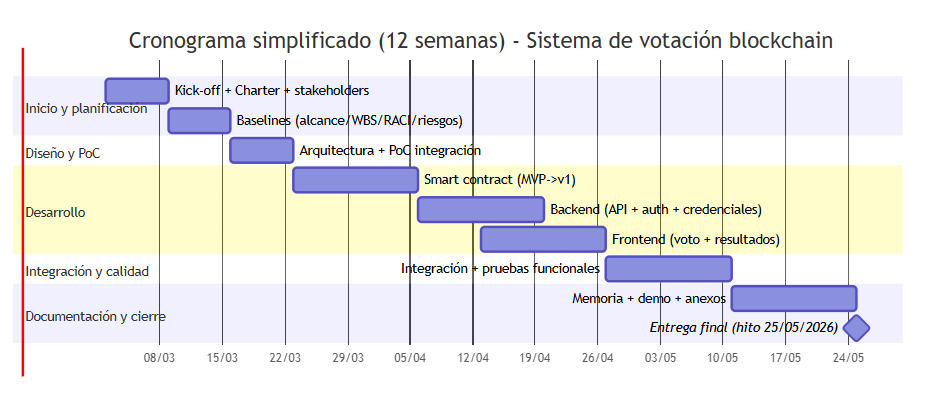
\includegraphics[width=0.95\linewidth]{images/cronograma.png}
% \caption{Cronograma simplificat del projecte}
% \label{fig:cronograma}
% \end{figure}

% \subsection{Fites del projecte}

% Les fites del projecte representen punts clau de control que permeten verificar el progrés, validar els lliurables i assegurar l’alineació amb els objectius establerts. Cada fita marca la finalització d’un resultat verificable i facilita el seguiment del cronograma, la gestió de riscos i la presa de decisions.

% Des d’una perspectiva de gestió de projectes alineada amb PMBOK, les fites constitueixen referències temporals essencials per monitoritzar l’estat del projecte, detectar desviacions i garantir que el desenvolupament avança de manera controlada i coherent amb el pla establert.

% A més, la definició de criteris de verificació per a cada fita assegura que els lliurables siguin objectivament avaluables i que el progrés del projecte pugui ser validat de forma transparent.

% \begin{table}[H]
% \centering
% \begin{tabular}{|p{5cm}|p{3cm}|p{6cm}|}
% \hline
% \textbf{Fita} & \textbf{Data} & \textbf{Criteri de verificació} \\
% \hline
% Project Charter aprovat & 08/03/2026 & Objectius i governança definits \\
% \hline
% Baseline d’abast & 15/03/2026 & WBS i abast validats \\
% \hline
% Arquitectura validada & 22/03/2026 & PoC funcional \\
% \hline
% Smart contract MVP & 29/03/2026 & Tests superats \\
% \hline
% Integració backend & 19/04/2026 & Flux de vot funcional \\
% \hline
% MVP end-to-end & 26/04/2026 & Vot i resultats operatius \\
% \hline
% Beta estable & 10/05/2026 & Proves completes \\
% \hline
% Documentació final & 24/05/2026 & Memòria i annexos complets \\
% \hline
% Entrega final & 25/05/2026 & Lliurament realitzat \\
% \hline
% \end{tabular}
% \caption{Fites principals del projecte}
% \end{table}


% \subsection{Assignació de responsabilitats}
% Per garantir una distribució clara de responsabilitats i una coordinació eficient entre els membres de l’equip, s’ha definit una matriu RACI (\textit{Responsible, Accountable, Consulted, Informed}). Aquesta eina permet identificar de manera precisa qui és responsable de l’execució de cada entregable, qui n’assumeix la responsabilitat final, quins membres han de ser consultats i qui ha de ser informat del seu progrés.

% L’ús de la matriu RACI facilita la comunicació interna, evita duplicitats de tasques i redueix ambigüitats en la presa de decisions. A més, constitueix una pràctica àmpliament utilitzada en la gestió de projectes, ja que contribueix a millorar la governança, la transparència i l’eficiència del treball col·laboratiu.

% En el context d’aquest projecte, la matriu RACI s’aplica als principals lliurables amb l’objectiu d’assegurar una assignació clara de rols i una execució coordinada de les activitats.

% \begin{table}[H]
% \centering
% \small
% \setlength{\tabcolsep}{6pt}
% \renewcommand{\arraystretch}{1.2}
% \begin{tabular}{|p{5cm}|c|c|c|c|}
% \hline
% \textbf{Entregable} & \textbf{PM} & \textbf{Backend} & \textbf{Frontend} & \textbf{QA} \\
% \hline
% Project Charter      & A   & C   & I   & C   \\
% Scope baseline       & A   & R   & R   & C   \\
% Cronograma           & A   & R   & C   & C   \\
% Costos               & A   & R   & C   & C   \\
% Riscos               & A   & C   & C   & R   \\
% Arquitectura         & A   & R   & R   & C   \\
% Smart contract       & C   & A/R & I   & R   \\
% Backend API          & C   & A/R & C   & R   \\
% Frontend             & C   & C   & A/R & R   \\
% Informe proves       & C   & C   & C   & A/R \\
% Memòria final        & A/R & C   & C   & C   \\
% Presentació          & A   & R   & R   & C   \\
% \hline
% \end{tabular}
% \caption{Matriu RACI del projecte}
% \end{table}


% %------------------------------------------------
% \subsection{Diagrama RACI}
% %------------------------------------------------

% El diagrama RACI proporciona una representació visual de la distribució de responsabilitats dins del projecte, complementant la matriu RACI presentada anteriorment. Aquesta representació facilita la comprensió immediata de qui executa cada activitat, qui n’assumeix la responsabilitat final i com es coordinen les tasques fins a l’entrega del sistema.

% El model RACI defineix els rols següents:

% \begin{itemize}
% \item \textbf{Responsible (R):} membre encarregat de l’execució directa de la tasca.
% \item \textbf{Accountable (A):} responsable final del resultat i de la presa de decisions.
% \item \textbf{Consulted (C):} membres que aporten coneixement i suport durant l’activitat.
% \item \textbf{Informed (I):} membres que han de ser informats del progrés o resultats.
% \end{itemize}

% El diagrama mostra el flux de responsabilitats des dels rols tècnics cap als lliurables principals i, finalment, cap a l’entrega del projecte.

% \subsubsection{Anàlisi del flux de responsabilitats}

% El desenvolupament tècnic es distribueix entre els especialistes de cada àrea:

% \begin{itemize}
% \item El \textbf{desenvolupador Back-end + Blockchain} és responsable de la implementació del \textit{smart contract}, component crític que garanteix la seguretat, integritat i immutabilitat del sistema.
% \item El \textbf{desenvolupador Front-end} és responsable de la interfície web i de la interacció amb la blockchain, assegurant una experiència d’usuari clara i funcional.
% \item L’àrea de \textbf{Qualitat (QA)} és responsable de les proves funcionals, la validació del sistema i la generació d’evidències i informes de resultats.
% \end{itemize}

% Aquestes activitats convergeixen en la fase d’integració end-to-end, on es verifica el funcionament complet del sistema.

% \subsubsection{Responsabilitat de governança}

% El \textbf{Project Manager} assumeix la responsabilitat final dels lliurables de planificació i governança, assegurant la coherència entre abast, temps i recursos, així com el compliment dels objectius del projecte.

% \subsubsection{Convergència cap a l’entrega final}

% El diagrama il·lustra com les diferents línies de treball convergeixen cap a dues fites principals:

% \begin{itemize}
% \item la validació tècnica del sistema mitjançant la integració end-to-end,
% \item la verificació funcional i documental a través de les proves i l’informe de qualitat.
% \end{itemize}

% Ambdues línies conflueixen en l’entrega final, garantint que el sistema sigui funcional, verificable i adequadament documentat.

% Aquest enfocament visual facilita la coordinació de l’equip, millora la comunicació interna i assegura una execució ordenada i transparent del projecte.

% \begin{figure}[H]
% \centering
% \begin{tikzpicture}[
% box/.style={rectangle, draw, rounded corners, align=center, minimum width=3cm, minimum height=1cm},
% arrow/.style={->, thick}
% ]

% % Roles
% \node[box] (pm) {Project\\Manager};
% \node[box, below=1.8cm of pm] (backend) {Backend +\\Blockchain};
% \node[box, below=1.8cm of backend] (frontend) {Front-end};
% \node[box, below=1.8cm of frontend] (qa) {QA};

% % Deliverables
% \node[box, right=3.5cm of pm] (planning) {Planificació\\i Governança};
% \node[box, below=3cm of planning] (integration) {Integració\\End-to-End};
% \node[box, right=3.5cm of qa] (testing) {Proves i\\Validació};
% \node[box, right=3cm of integration] (delivery) {Entrega\\Final};

% % Arrows
% \draw[arrow] (backend) -- (integration);
% \draw[arrow] (frontend) -- (integration);
% \draw[arrow] (qa) -- (testing);
% \draw[arrow] (integration) -- (delivery);
% \draw[arrow] (testing) -- (delivery);
% \draw[arrow] (pm) -- (planning);
% \draw[arrow] (planning) -- (delivery);

% \end{tikzpicture}
% \caption{Diagrama RACI simplificat del flux de responsabilitats}
% \end{figure}

% \subsection{Camí crític i dependències}

% El camí crític representa la seqüència d’activitats que determina la durada total del projecte. Aquestes tasques no disposen de marge temporal i qualsevol retard en la seva execució pot afectar directament la data final d’entrega.

% En aquest projecte, el camí crític està format per:

% \begin{itemize}
% \item el desenvolupament del \textit{smart contract}, nucli funcional que garanteix la integritat i seguretat del sistema,
% \item la integració amb el backend, necessària per gestionar credencials i executar el flux de vot,
% \item la integració amb el frontend, que permet la interacció de l’usuari amb el sistema,
% \item les proves end-to-end, imprescindibles per verificar el funcionament complet de la solució.
% \end{itemize}

% Aquestes activitats constitueixen la columna vertebral del projecte i requereixen un seguiment prioritari per evitar desviacions en el calendari.

% \subsection{Gestió de reserves i incertesa}

% En la planificació del projecte s’ha previst una reserva temporal durant l’última setmana, amb l’objectiu de gestionar possibles imprevistos i reduir el risc associat a la fase final d’integració.

% Aquesta reserva permet abordar:

% \begin{itemize}
% \item incidències tècniques inesperades,
% \item ajustos derivats de la integració final,
% \item millores d’usabilitat i estabilitat,
% \item revisió i millora de la qualitat de la documentació.
% \end{itemize}

% La incorporació d’aquest buffer temporal constitueix una pràctica habitual en la gestió de projectes, ja que permet absorbir la incertesa inherent als sistemes tecnològics i augmenta la probabilitat d’assolir els objectius dins del termini establert.

% %------------------------------------------------
% \section{Metodologia d’estimació de l’esforç}
% %------------------------------------------------

% L’estimació de l’esforç del projecte s’ha realitzat mitjançant un enfocament sistemàtic i replicable, amb l’objectiu d’obtenir una previsió realista i coherent amb l’abast funcional, la planificació temporal i la complexitat tècnica del sistema.

% S’adopta un enfocament combinat basat en bones pràctiques de gestió de projectes:

% \begin{itemize}
% \item \textbf{Descomposició WBS (Work Breakdown Structure) amb enfocament bottom-up:} el projecte es divideix en paquets de treball (entregables), s’estimen les hores per paquet i l’agregació proporciona l’esforç total.
% \item \textbf{Estimació PERT en tasques d’alta incertesa:} aplicada als smart contracts i a la integració tècnica per reflectir aprenentatge, risc i variabilitat.
% \item \textbf{Reserva de contingència:} destinada a cobrir riscos identificats durant l’anàlisi tècnica.
% \item \textbf{Reserva de gestió:} destinada a imprevistos no identificats durant la planificació.
% \end{itemize}

% \subsection{Estimació PERT}

% Per als paquets amb major incertesa s’utilitza el mètode PERT, que considera tres escenaris:

% \begin{itemize}
% \item O (Optimista)
% \item M (Més probable)
% \item P (Pessimista)
% \end{itemize}

% L’estimació ponderada es calcula mitjançant:

% \[
% E = \frac{O + 4M + P}{6}
% \]

% Aquest mètode permet reflectir el risc tècnic associat a tecnologies noves com els smart contracts i la seva integració.

% \begingroup
% \begin{table}[H]
% \centering
% \footnotesize
% \begin{tabular}{|p{4cm}|c|c|c|c|}
% \hline
% \textbf{Paquet de treball} & \textbf{O} & \textbf{M} & \textbf{P} & \textbf{Estimació PERT (h)} \\
% \hline
% Smart contract (lògica de vot) & 24 & 36 & 60 & 38 \\
% \hline
% Integració blockchain–backend & 16 & 24 & 40 & 25 \\
% \hline
% Connexió wallet i validació & 10 & 16 & 28 & 17 \\
% \hline
% \end{tabular}
% \caption{Estimació PERT en paquets d’alta incertesa}
% \end{table}
% \endgroup

% \subsection{Esforç base del projecte}

% El projecte parteix d’una estimació base de \textbf{245 hores-persona}, que inclou:

% \begin{itemize}
% \item investigació i aprenentatge tecnològic,
% \item disseny d’arquitectura,
% \item desenvolupament de smart contracts,
% \item desenvolupament back-end,
% \item desenvolupament front-end,
% \item integració del sistema,
% \item proves i validació,
% \item documentació i presentació.
% \end{itemize}

% Aquesta estimació constitueix la base per a la planificació del treball i la distribució de càrrega entre rols.

% \subsection{Distribució d’esforç per rol}


% \begin{table}[H]
% \footnotesize
% \centering
% \begin{tabular}{|l|c|c|p{7cm}|}
% \hline
% \textbf{Rol} & \textbf{Hores} & \textbf{\%} & \textbf{Justificació} \\
% \hline
% Project Manager & 47 & 19\% & Planificació, coordinació, coherència documental i tancament del projecte. \\
% \hline
% Desenvolupador Back-end + Blockchain & 107 & 44\% & Desenvolupament del nucli tècnic: smart contracts, API i integració. \\
% \hline
% Desenvolupador Front-end & 48 & 20\% & Desenvolupament de la interfície d’usuari i integració web3. \\
% \hline
% Qualitat i Validació (QA) & 43 & 18\% & Proves, control de qualitat, evidències i suport a la integració. \\
% \hline
% \textbf{Total} & \textbf{245} & \textbf{100\%} & \\
% \hline
% \end{tabular}
% \caption{Distribució estimada de l’esforç per rol}
% \end{table}

% \subsection{Reserves d’esforç}

% Per millorar la robustesa de la planificació s’incorporen reserves:

% \begin{itemize}
% \item \textbf{Contingència (10\%):} cobreix riscos identificats com la corba d’aprenentatge, dificultats d’integració o ajustos de seguretat.
% \item \textbf{Reserva de gestió (5\%):} cobreix imprevistos no identificats durant la planificació.
% \end{itemize}

% \[
% Esforç\ total\ previst = 245h + 10\% + 5\% \approx 282h
% \]

% Aquest marge incrementa la fiabilitat de la planificació sense comprometre el calendari.

% \section{Riscos i limitacions}

% La identificació i gestió de riscos constitueix un element essencial en la planificació del projecte, ja que permet anticipar possibles dificultats i establir estratègies per reduir-ne l’impacte.

% \subsection*{Riscos tècnics}
% \begin{itemize}
%     \item complexitat en el desenvolupament dels \textit{smart contracts},
%     \item gestió segura de claus criptogràfiques i credencials,
%     \item necessitat de garantir simultàniament anonimat i verificabilitat del vot.
% \end{itemize}

% \subsection*{Riscos de projecte}
% \begin{itemize}
%     \item corba d’aprenentatge associada a la tecnologia blockchain,
%     \item dificultats derivades de la integració de tecnologies noves.
% \end{itemize}

% \subsection*{Estratègies de mitigació}
% \begin{itemize}
%     \item desenvolupament incremental per validar components crítics de forma progressiva,
%     \item ús d’eines i frameworks consolidats per reduir incertesa tècnica,
%     \item proves contínues per detectar errors en fases primerenques.
% \end{itemize}


% \section{Resultats esperats}

% En finalitzar el projecte s’espera disposar d’un prototip funcional que demostri la viabilitat d’un sistema de votació electrònica basat en blockchain.

% Concretament, s’espera obtenir:

% \begin{itemize}
%     \item un sistema funcional de votació blockchain,
%     \item una demostració pràctica operativa del procés de votació,
%     \item \textit{smart contracts} funcionals i verificables,
%     \item documentació tècnica completa del sistema desenvolupat,
%     \item coneixement pràctic sobre blockchain i contractes intel·ligents.
% \end{itemize}

% Aquests resultats permetran validar tant els objectius tècnics com els objectius formatius del projecte.

\section{Arquitectura de la solució}
 
Aquesta secció descriu l'arquitectura tècnica del sistema de votació electrònica descentralitzat. L'objectiu és presentar una visió completa dels components del sistema, les seves responsabilitats, les relacions entre ells i les decisions de disseny que justifiquen cada elecció. L'arquitectura segueix el model C4 de Simon Brown, que permet representar el sistema a quatre nivells de detall creixent: context, contenidors, components i codi.
 
El principi fonamental que guia tot el disseny és l'eliminació del punt únic de fallada. Cap component individual del sistema ha de tenir la capacitat de modificar, censurar o invalidar un vot per si sol. Aquesta propietat es garanteix per construcció arquitectònica: la lògica electoral resideix íntegrament dins un contracte intel·ligent immutable desplegat a la xarxa Algorand, i cap servidor intermedi té accés a les claus privades dels votants ni al codi executable del contracte.

\href{https://drive.google.com/file/d/19bZjOcyCW3vcCqPl0YcqOhWvxd-m8CH3/view?usp=sharing}{URL diagrama.}
 
\subsection{Visió general del sistema (Nivell 1 --- Context)}
 
El diagrama de context identifica els actors i sistemes externs que interactuen amb el sistema de votació descentralitzat:
 
\begin{enumerate}[label=\roman*.]
    \item \textbf{Votant}: persona física que emet el seu vot o proposa una elecció a través de la interfície web. Constitueix l'actor principal del sistema i l'únic que genera transaccions de votació.
    \item \textbf{Pera Wallet}: sistema de \textit{software} extern que gestiona les claus privades del votant. El sistema mai accedeix directament a aquestes claus; tota signatura criptogràfica es delega exclusivament a la cartera digital mitjançant el protocol WalletConnect.
    \item \textbf{Full Node Algorand}: servidor hostatjat per la universitat (o per les entitats institucionals participants) que rep les transaccions de l'aplicació i les propaga per la xarxa blockchain. La comunicació entre l'aplicació i el node es realitza via TCP/IP. En el diagrama de context, el node es representa com un sistema extern al \textit{software} del sistema de votació, ja que la seva implementació correspon al protocol natiu d'Algorand (Go) i no al codi desenvolupat per l'equip del projecte.
    \item \textbf{Xarxa Ethereum}: emprada exclusivament com a notari públic. Un cop tancada l'elecció, el servei d'anchoring calcula el \textit{hash} SHA-256 de l'estat final de l'escrutini i l'envia a un contracte intel·ligent propi desplegat a Ethereum (Sepolia Testnet) que implementa un mecanisme de consens amb llindar, garantint un ancoratge immutable i auditable de manera independent.
\end{enumerate}
 
Les comunicacions entre actors segueixen protocols estàndard: la interfície web es connecta al node Algorand via HTTPS/REST, la signatura dels vots es gestiona mitjançant WalletConnect, i l'ancoratge a Ethereum s'executa via JSON-RPC (Web3).

\begin{figure}[H]
    \centering
    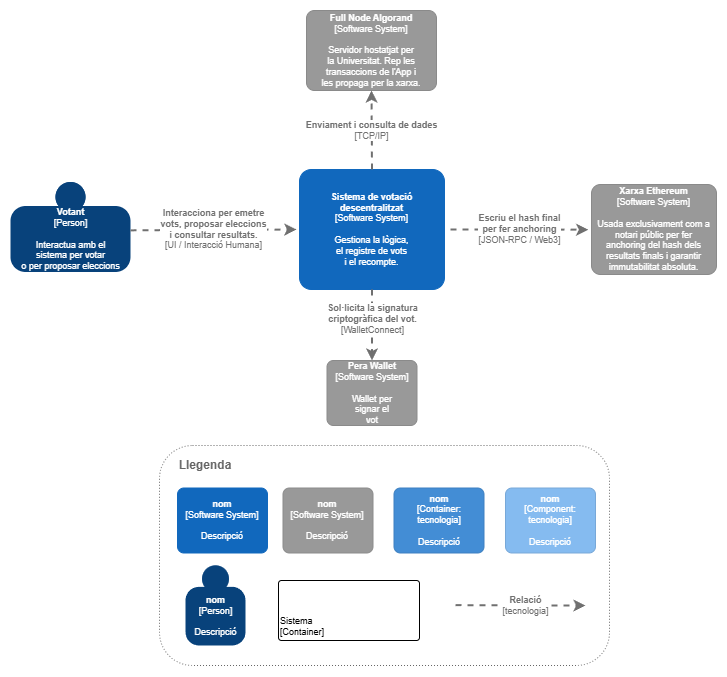
\includegraphics[width=0.85\textwidth]{images/c4-n1.png} 
    \caption{Diagrama de context del sistema (Nivell 1 del model C4).}
    \label{fig:c4-nivell-1}
\end{figure}
 
\subsection{Contenidors del sistema (Nivell 2)}
 
El sistema es descompon en cinc contenidors principals, cadascun amb una responsabilitat ben delimitada i un acoblament mínim amb la resta:
 
\subsubsection{Aplicació web \textit{(\textit{front-end}})}
 
Aplicació d'una sola pàgina (\textit{Single-Page Application}) que el votant descarrega des d'un repositori oficial i executa localment. Desenvolupada amb React i empaquetada amb Vite, és responsable de renderitzar la interfície d'usuari, mostrar les eleccions actives, empaquetar el vot en format de transacció Algorand (ApplicationCall) i enviar-lo al node. L'aplicació no emmagatzema cap dada sensible i opera com un client lleuger (\textit{thin client}) que delega tota la lògica de negoci al contracte intel·ligent.
 
El flux d'interacció de l'usuari segueix una seqüència de quatre passos: (1) l'usuari ordena els candidats per preferència mitjançant \textit{drag and drop}, (2) l'aplicació empaqueta l'ordre de preferències en format de transacció Algorand, (3) sol·licita la signatura criptogràfica a la cartera digital i (4) envia la transacció signada al node complet d'Algorand perquè la propagui a la xarxa.

 
\subsubsection{Node Complet d'Algorand}
 
Servidor hostatjat per la universitat (o, en un escenari productiu, per les entitats institucionals participants) que rep les transaccions de l'aplicació web i les propaga per la xarxa blockchain. Implementat en Go, exposa una API REST estàndard compatible amb l'Algorand SDK. La seva funció és exclusivament la de punt d'entrada a la xarxa: no conté lògica de negoci pròpia ni té accés a les claus dels votants.
 
 
\subsubsection{Smart Contract de Votació}
 
Lògica immutable desplegada a la xarxa Algorand, escrita en PyTeal i compilada a TEAL (Transaction Execution Approval Language). Constitueix el nucli del sistema i la peça que elimina la necessitat de confiança en cap autoritat central. Les seves responsabilitats són:
 
\begin{enumerate}[label=\roman*.]
    \item Votacions d'eleccions.
    \item Generació i emmagatzematge de propostes d'eleccions.
    \item Validació del cens electoral i verificació de permisos (verificació que l'adreça del votant pertany a la llista blanca i que l'acció sol·licitada pot ser realitzada).
    \item Prevenció del doble vot.
    \item Gestió del cicle de vida de l'elecció (dates d'inici i finalització).
    \item Recompte automàtic i transparent dels vots.
\end{enumerate}
 
L'estat del contracte s'emmagatzema emprant dos mecanismes natius d'Algorand: \textbf{Box Storage} per guardar les propostes i el recompte global de vots, i \textbf{Global State} per registrar si un votant concret ja ha exercit el seu dret, evitant així el doble vot sense revelar l'opció seleccionada.
 
\subsubsection{Servei d'Anchoring}
 
Component automatitzat que cada entitat que opera un node complet (\textit{full node}) ha d'executar. Aquest servei llegeix l'estat de les votacions des del node d'Algorand via l'AlgoSDK REST API i, quan una elecció finalitza, genera el \textit{hash} SHA-256 de l'estat de la blockchain corresponent a l'escrutini. Seguidament, envia aquest \textit{hash} signat a un contracte intel·ligent propi desplegat a la xarxa pública d'Ethereum (Sepolia Testnet) mitjançant JSON-RPC.

El contracte d'Ethereum (escrit en Solidity) actua com una ``cort suprema'' descentralitzada: manté una llista blanca d'adreces de wallet universitàries autoritzades i implementa una lògica de consens amb llindar (\textit{\textit{K-of-N}}). Només quan K universitats independents acorden un \textit{hash} d'estat idèntic, el contracte ancora el resultat final de l'elecció al registre d'Ethereum, evitant així el frau per punt únic de fallada.

\subsubsection{Pera Wallet (sistema extern)}
 
Cartera digital mòbil de l'ecosistema Algorand que actua com a custòdia exclusiva de les claus privades del votant. El sistema interactua amb Pera Wallet a través del protocol WalletConnect: l'aplicació web genera un codi QR, l'usuari l'escaneja, i la cartera retorna la transacció signada criptogràficament sense que la clau privada abandoni mai el dispositiu mòbil de l'elector.

\begin{figure}[H]
    \centering
    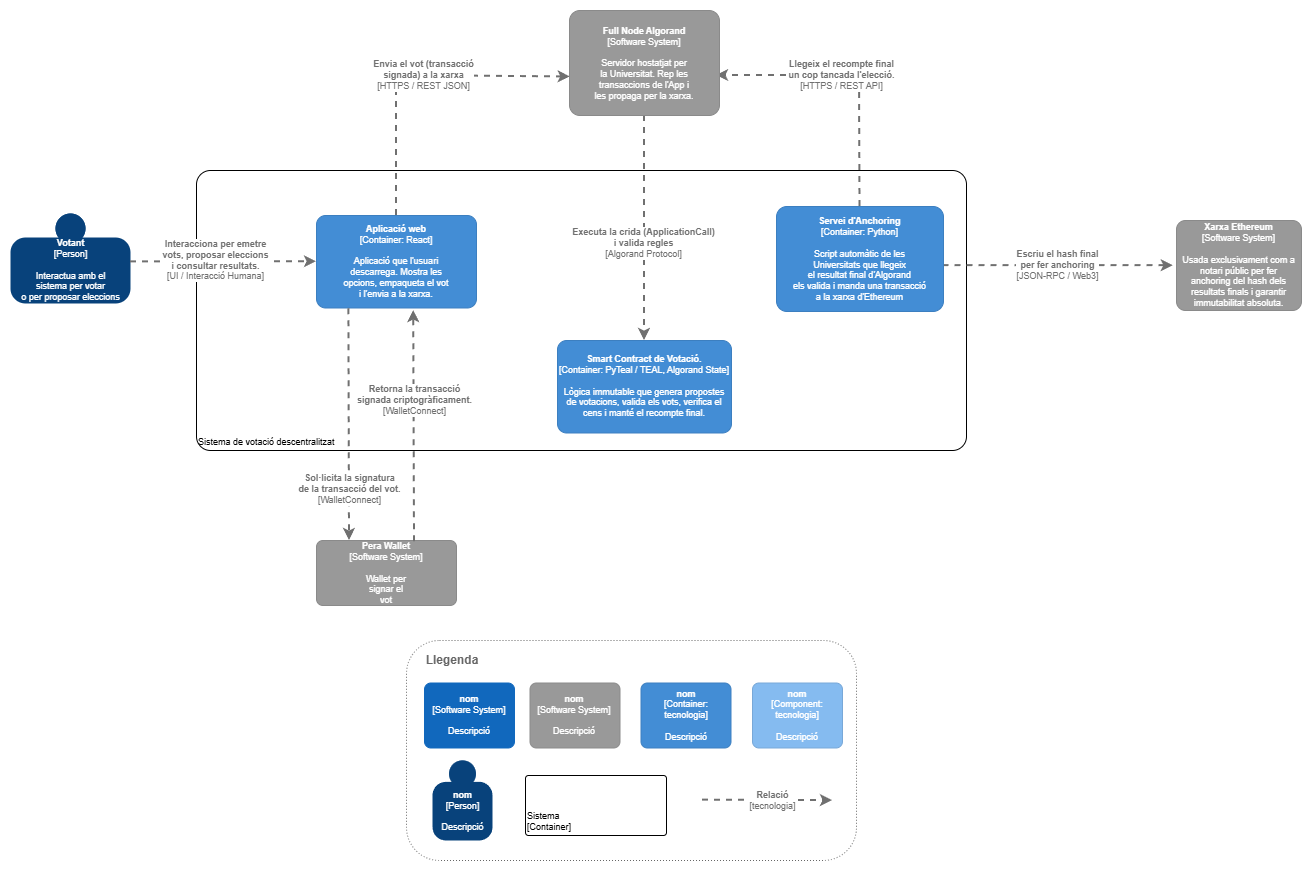
\includegraphics[width=0.85\textwidth]{images/c4-n2.png} 
    \caption{Diagrama de contenidors del sistema (Nivell 2 del model C4).}
    \label{fig:c4-nivell-2}
\end{figure}

\subsection{Components interns (Nivell 3)}
 
A continuació es detalla la descomposició interna dels tres contenidors desenvolupats per l'equip del projecte: l'aplicació web, el contracte intel·ligent i el servei d'anchoring.
 
\subsubsection{Components de l'aplicació web}

L'aplicació React es descompon en quatre capes principals amb responsabilitats clarament separades:

\begin{enumerate}[label=\roman*.]
    \item \textbf{Capa de presentació} (\textit{React Components}): conté set vistes (\texttt{Landing}, \texttt{Dashboard}, \texttt{Elections}, \texttt{Proposals}, \texttt{Voting}, \texttt{Results} i \texttt{Verification}), cadascuna amb els seus propis fitxers JSX i CSS. Els components reutilitzables d'interfície (\texttt{Button}, \texttt{Card}, \texttt{DraggableList}, \texttt{Timeline}, \texttt{DotGrid}) i els de disposició (\texttt{Navbar}, \texttt{PageWrapper}) s'agrupen per separat. El disseny segueix una estètica \textit{glassmorphism} amb mode clar i fosc.

    \item \textbf{Capa d'internacionalització} (\textit{react-i18next}): tota la interfície està disponible en anglès, espanyol i català mitjançant fitxers de traducció JSON. El sistema detecta automàticament l'idioma del navegador i permet canviar-lo manualment des de la barra de navegació.

    \item \textbf{Mòdul WalletConnect} (\textit{WalletConnect SDK}): gestiona la sessió amb Pera Wallet, genera el codi QR per establir la connexió i envia les sol·licituds de signatura a l'usuari. Encapsula tota la complexitat del protocol de comunicació amb la cartera.

    \item \textbf{Generador de transaccions} (\textit{Algorand JS SDK --- algosdk}): tradueix les accions de l'usuari (``Votar opció A'' o ``Proposar elecció X'') en transaccions \textit{byte-code} d'Algorand (ApplicationCall) a punt per ser signades. Aquesta capa d'abstracció garanteix que la resta de l'aplicació no necessita conèixer els detalls de baix nivell del protocol Algorand.
\end{enumerate}

El flux de navegació de l'aplicació comença amb una pàgina d'aterratge (\texttt{Landing}), des de la qual l'usuari accedeix al tauler de control (\texttt{Dashboard}). Des d'allà pot consultar eleccions actives i passades (\texttt{Elections}), redactar propostes (\texttt{Proposals}), emetre el seu vot mitjançant un sistema D\&D amb mètode Schulze (\texttt{Voting}), consultar resultats amb la matriu de comparació per parells (\texttt{Results}) i verificar el seu vot a la cadena de blocs (\texttt{Verification}).

La capa de presentació sol·licita accions al generador de transaccions, que construeix la transacció i demana la signatura al mòdul WalletConnect. Un cop la cartera retorna la transacció signada, el generador l'envia directament al node complet d'Algorand mitjançant HTTPS/REST JSON.

\begin{figure}[H]
    \centering
    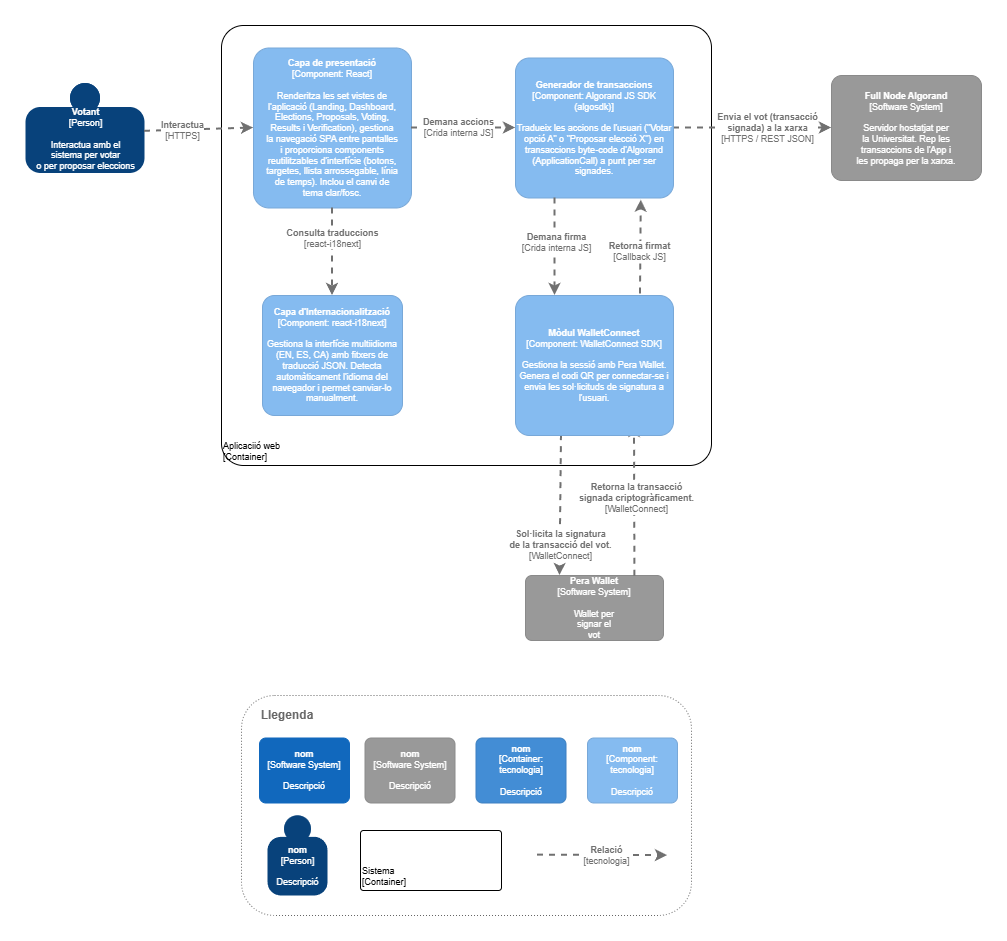
\includegraphics[width=0.85\textwidth]{images/c4-n3-app.png} 
    \caption{Components de l'aplicació web (Nivell 3 del model C4).}
    \label{fig:c4-nivell-3-app}
\end{figure}


\subsubsection{Components del Smart Contract}
 
El contracte intel·ligent es descompon internament en sis mòduls lògics. La interacció entre el node Algorand i el contracte segueix l'estàndard ABI d'Algorand (ARC-4), que defineix la codificació dels arguments i els valors de retorn de cada crida:
 
\begin{enumerate}[label=\roman*.]
    \item \textbf{Enrutador principal} (\textit{PyTeal Cond}): punt d'entrada del contracte. Rep cada transacció i, segons els arguments de l'ApplicationCall, la redirigeix al mòdul de votació, al de propostes o al generador d'eleccions. Implementa el patró \textit{Router} per centralitzar el control del flux d'execució.

    \item \textbf{Verificador} (\textit{PyTeal}): encarregat de verificar que l'acció sol·licitada a la transacció pugui ser realitzada. Comprova que l'acció no s'hagi realitzat amb anterioritat (per exemple, que l'usuari no hagi votat ja) i revisa que la \textit{wallet} que ha signat la transacció tingui permisos per executar l'operació sol·licitada (pertinença al cens). La comunicació amb l'emmagatzematge d'estat es fa mitjançant les operacions \texttt{box\_get()} del protocol Box Opcode d'Algorand. L'enrutador delega la validació a aquest mòdul mitjançant crides internes (\texttt{CallSub}).

    \item \textbf{Lògica de propostes} (\textit{PyTeal}): encarregat de comunicar-se amb l'estat del contracte per registrar una proposta d'elecció. Defineix les dates d'inici i finalització, el nom de la proposta, els participants i les entitats o opcions a ser elegides. L'escriptura a l'estat es realitza mitjançant actualitzacions atòmiques (\texttt{app\_global\_put()}).

    \item \textbf{Lògica de votació} (\textit{PyTeal}): encarregat de comunicar-se amb l'estat del contracte per modificar el recompte de vots. L'escriptura d'increments de vot es fa mitjançant actualitzacions atòmiques (\texttt{app\_global\_put()}) que garanteixen la consistència de l'estat.

    \item \textbf{Generador d'eleccions} (\textit{PyTeal}): llegeix l'estat del contracte (els vots de les propostes d'eleccions mitjançant \texttt{box\_get()}) i, si una proposta ha assolit un llindar determinat de vots favorables, genera automàticament les eleccions corresponents mitjançant transaccions internes (\texttt{itxn.submit()}). Implementa la lògica de transició entre la fase de proposta i la fase electoral. La lògica de propostes notifica aquest mòdul mitjançant \texttt{CallSub()} cada cop que es registra un nou vot a una proposta.

    \item \textbf{Emmagatzematge d'estat} (\textit{Algorand Box Storage \& Local State}): base de dades del contracte. Guarda les propostes (Box Storage), el recompte de vots per proposta, el recompte de vots per elecció (Global/Box) i el registre individual de qui ha votat (Local State per evitar el doble vot).
\end{enumerate}

\begin{figure}[H]
    \centering
    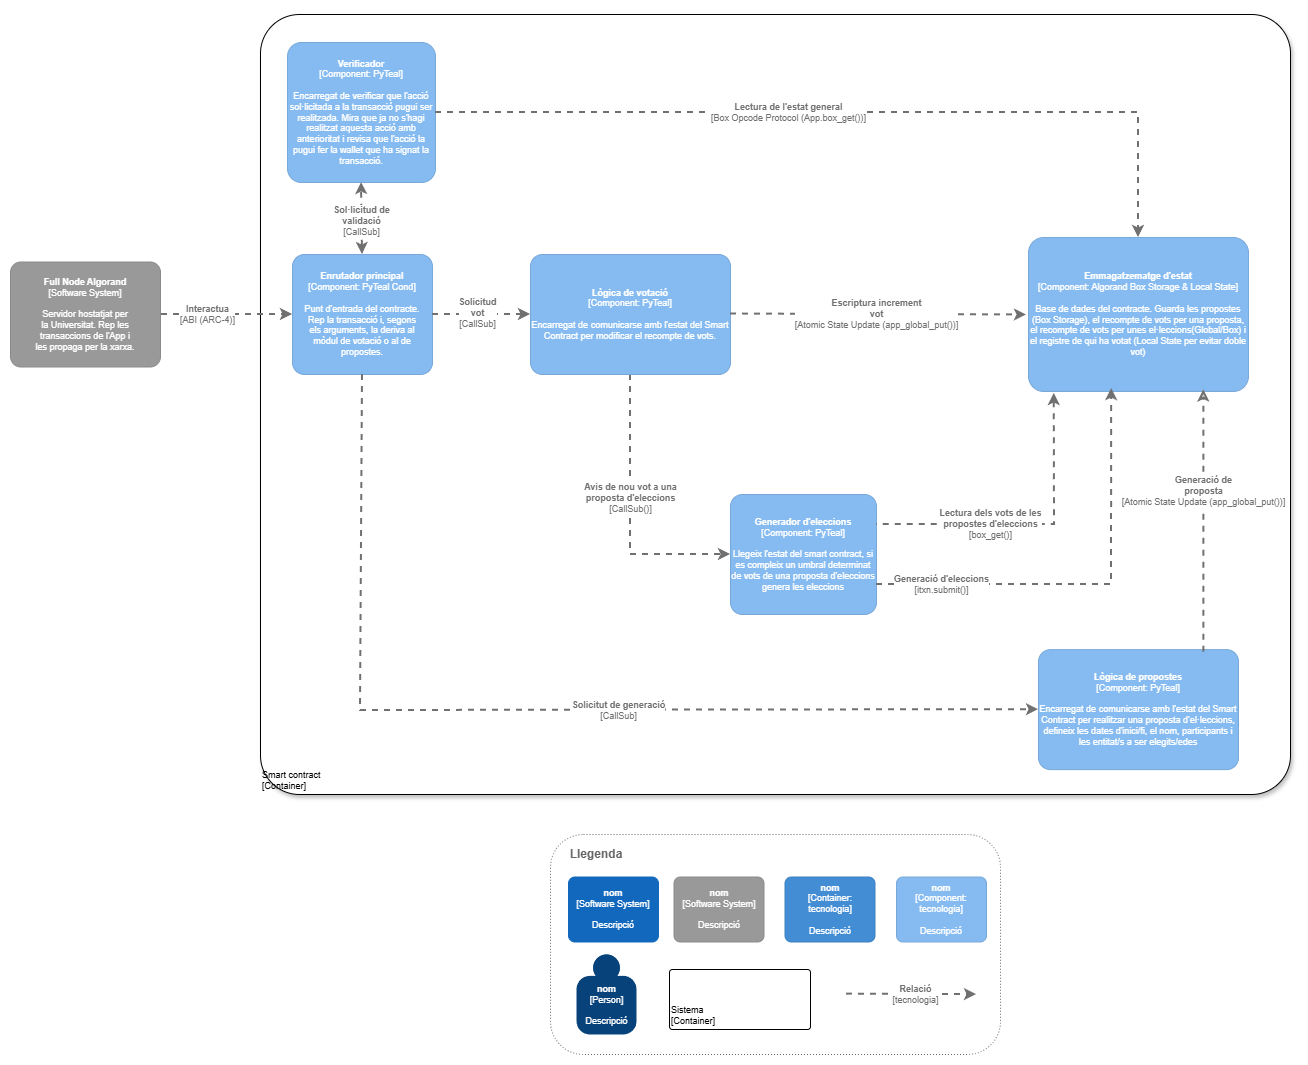
\includegraphics[width=0.85\textwidth]{images/c4-n3-smart-contract.png} 
    \caption{Components del Smart Contract (Nivell 3 del model C4).}
    \label{fig:c4-nivell-3-sc}
\end{figure}

\subsubsection{Components del Servei d'Anchoring}

El servei d'anchoring es descompon en dos components que operen conjuntament per materialitzar l'ancoratge distribuït dels resultats:

\begin{enumerate}[label=\roman*.]
    \item \textbf{Gestor d'ancoratge} (\textit{Python}): mòdul encarregat de revisar l'estat de les votacions consultant el node d'Algorand via l'AlgoSDK REST API. Quan una votació finalitza, aquest component genera el \textit{hash} SHA-256 de l'estat de la blockchain corresponent a l'escrutini i l'envia, signat criptogràficament (ECDSA), al contracte d'Ethereum mitjançant JSON-RPC.

    \item \textbf{Ethereum Notary Contract} (\textit{Solidity}): contracte intel·ligent desplegat a la xarxa Ethereum (Sepolia Testnet), dissenyat i implementat pel propi equip del projecte. Actua com una ``cort suprema'' descentralitzada que manté una \textit{whitelist} d'adreces de wallet universitàries autoritzades i implementa una lògica de consens amb llindar (\textit{\textit{K-of-N}}). Agrega els \textit{hash}es d'estat provinents dels nodes universitaris i només ancora el resultat final de l'elecció al registre d'Ethereum quan K universitats independents acorden un \textit{hash} d'estat idèntic, evitant així el frau per punt únic de fallada. Les funcionalitats del contracte inclouen: mantenir la llista d'adreces autoritzades (afegir i eliminar), rebre transaccions dels nodes autoritzats i, si se supera el llindar de coincidència, publicar el \textit{hash} a la xarxa.
\end{enumerate}

\begin{figure}[H]
    \centering
    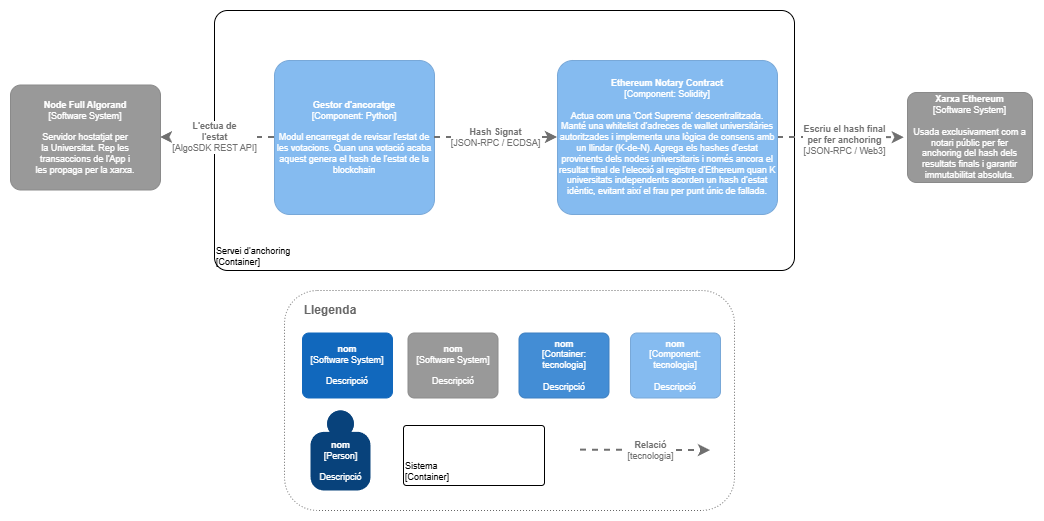
\includegraphics[width=0.85\textwidth]{images/c4-n3-servei-anchoring.png} 
    \caption{Components del Servei d'Anchoring (Nivell 3 del model C4).}
    \label{fig:c4-nivell-3-anchoring}
\end{figure}


% ===========================================================================
%   SECCIÓ 9 - TECNOLOGIES I SOFTWARE DE TERCERS
% ===========================================================================
\section{Tecnologies i software de tercers}
 
El sistema s'ha construït emprant exclusivament eines de codi obert i plataformes gratuïtes, en coherència amb el requisit de projecte d'incórrer en zero despesa econòmica (secció 3.3.3 del document d'abast). Cada tecnologia s'ha seleccionat atenent a criteris de maduresa, documentació disponible, compatibilitat amb l'ecosistema Algorand i accessibilitat per a l'equip de desenvolupament. A continuació es descriuen les tecnologies emprades, agrupades per capa del sistema.
 
\subsection{Capa de blockchain i contractes intel·ligents}
 
\subsubsection{Algorand (protocol de consens)}
 
Algorand és la xarxa blockchain seleccionada com a infraestructura del sistema de votació. Utilitza un mecanisme de consens basat en Pure Proof of Stake (PPoS) combinat amb una Funció Aleatòria Verificable (VRF) que garanteix que la selecció de validadors és aleatòria, impredictible i verificable criptogràficament. Les seves propietats fonamentals per al projecte són: finalitat immediata de les transaccions (sense possibilitat de \textit{forks}), comissions de transacció negligibles (0,001 ALGO), i suport natiu per a contractes intel·ligents amb emmagatzematge d'estat (Global State, Local State i Box Storage).
 
La decisió d'emprar Algorand en lloc d'Ethereum per a la lògica de votació es justifica per tres raons: (1) la finalitat instantània elimina la incertesa sobre si un vot ha estat confirmat, (2) el cost per transacció és ordres de magnitud inferior al gas d'Ethereum, fent viable un sistema on cada vot és una transacció, i (3) el model d'emmagatzematge natiu (Box Storage) permet estructures de dades complexes directament al contracte sense necessitat de mapejar tot a \textit{storage slots} de 256 bits.
 
\subsubsection{PyTeal / TEAL}
 
PyTeal és una llibreria de Python que permet escriure contractes intel·ligents per a Algorand emprant sintaxi Python nativa, que posteriorment es compila a TEAL (\textit{Transaction Execution Approval Language}), el llenguatge d'assembler de la màquina virtual d'Algorand (AVM). L'elecció de PyTeal per sobre d'alternatives com Puya (Algorand Python) es basa en la major maduresa de la seva documentació i la disponibilitat d'exemples dins la comunitat, factors crítics donada la corba d'aprenentatge prevista a la gestió de riscos (secció 6.4).
 
Tot el codi dels contractes (lògica de propostes, votació, verificació, generació d'eleccions i enrutament) s'escriu en PyTeal i es compila a TEAL abans del desplegament. La interacció amb el contracte segueix l'estàndard ABI d'Algorand (ARC-4), que defineix la codificació dels arguments de cada crida. Aquesta separació entre el llenguatge de desenvolupament (Python) i el d'execució (TEAL) facilita les proves unitàries i la lectura del codi per part d'auditors.
 
\subsubsection{AlgorKit (AlgoKit)}
 
AlgorKit és l'eina oficial de la Fundació Algorand per a la gestió del cicle de vida complet dels projectes blockchain: creació de l'entorn local, desplegament de contractes, execució de proves i interacció amb la xarxa. En el context d'aquest projecte, s'empra per aixecar una xarxa Algorand local simulada dins un contenidor Docker amb una única comanda, permetent iterar ràpidament sobre el codi dels contractes sense incórrer en costos de xarxa.
 
AlgorKit proporciona comptes prefabricats amb saldos de prova, un indexer local per a consultes, i una CLI que automatitza les tasques repetitives de desplegament. Constitueix la peça clau per complir el requisit de reproducibilitat (secció 3.2.1): qualsevol membre de l'equip pot replicar l'entorn exacte clonant el repositori i executant \texttt{algokit localnet start}.

\subsubsection{Solidity (contracte d'Ethereum)}

Solidity és el llenguatge de programació emprat per escriure el contracte intel·ligent d'ancoratge desplegat a la xarxa Ethereum (Sepolia Testnet). Aquest contracte, denominat \textit{Ethereum Notary Contract}, implementa la lògica de consens amb llindar \textit{K-of-N} que agrega els \textit{hash}es enviats pels nodes universitaris. S'ha seleccionat Solidity per ser el llenguatge estàndard i més madur de l'ecosistema Ethereum, amb àmplia documentació i suport d'eines de desenvolupament com Hardhat o Remix.
 
\subsection{Capa de \textit{front-end}}
 
\subsubsection{React}
 
React (versió 19) és la llibreria de JavaScript seleccionada per al desenvolupament de la interfície d'usuari. La seva arquitectura basada en components reactius i el seu model de flux de dades unidireccional permeten mantenir una separació neta entre la presentació visual i la lògica d'estat de l'aplicació. L'equip compta amb experiència prèvia en React, la qual cosa redueix la corba d'aprenentatge i permet concentrar l'esforç en la integració \textit{blockchain}.
 
\subsubsection{Vite}
Vite és l'eina de construcció (\textit{build tool}) i servidor de desenvolupament emprada per al \textit{front-end}. Substitueix la configuració tradicional basada en Webpack i Create React App, oferint arrancades quasi instantànies gràcies al seu mode de servei basat en mòduls ES natius i una compilació de producció optimitzada mitjançant Rollup. El contenidor Docker del \textit{front-end} utilitza Bun com a \textit{runtime} alternatiu a Node.js per accelerar la instal·lació de dependències i l'execució del servidor de desenvolupament.

\subsubsection{react-i18next}
El sistema d'internacionalització es basa en la llibreria \texttt{react-i18next} combinada amb \texttt{i18next-browser-languagedetector}. Tota la interfície està disponible en tres idiomes (anglès, espanyol i català) mitjançant fitxers de traducció JSON separats per \textit{locale}. El detector d'idioma identifica automàticament la preferència del navegador de l'usuari i permet el canvi manual d'idioma des de la barra de navegació.
 
\subsubsection{Algorand JavaScript SDK (algosdk)}
 
La llibreria oficial \texttt{algosdk} permet a l'aplicació web construir, signar i enviar transaccions d'Algorand des del navegador. S'empra per traduir les accions de l'usuari en transaccions \textit{ApplicationCall} byte-code compatibles amb el contracte intel·ligent, seguint l'estàndard ABI (ARC-4). La versió emprada suporta la construcció de transaccions atòmiques (grups de transaccions) i la interacció amb Box Storage.
 
\subsubsection{WalletConnect SDK}
 
WalletConnect és el protocol de comunicació estàndard entre aplicacions web (dApps) i carteres digitals mòbils. El SDK s'integra a l'aplicació React per generar codis QR de connexió, establir sessions xifrades amb Pera Wallet i enviar sol·licituds de signatura. Totes les comunicacions entre l'aplicació i la cartera es xifren mitjançant un pont (\textit{bridge}) independent, garantint que la clau privada del votant mai transita per la xarxa de l'aplicació.
 
\subsection{Capa d'anchoring i auditoria}
 
\subsubsection{Ethereum (Sepolia Testnet)}
 
La xarxa pública d'Ethereum s'empra exclusivament com a notari públic extern. El servei d'anchoring de cada node institucional envia el \textit{hash} SHA-256 dels resultats finals al contracte d'Ethereum Notary desplegat a la Sepolia Testnet, que aplica la lògica de consens amb llindar abans de publicar el resultat. La selecció de Sepolia en lloc d'altres testnets (Goerli, ja obsoleta) segueix la recomanació oficial de la Fundació Ethereum per a aplicacions de prova.
 
\subsubsection{Web3.py}
 
Llibreria de Python que proporciona la interfície de comunicació amb la xarxa Ethereum mitjançant el protocol JSON-RPC. S'empra dins el gestor d'ancoratge per construir i enviar la transacció que conté el \textit{hash} de l'escrutini al contracte Notary. La seva compatibilitat nativa amb Sepolia i la seva àmplia documentació la fan la solució més directa per a l'escriptura de dades a Ethereum des d'un script Python.
 
\subsection{Capa d'infraestructura i desplegament}
 
\subsubsection{Docker}
 
Docker és l'eina central de contenidorització del projecte. Permet empaquetar tots els serveis del sistema (node Algorand, servidor \textit{front-end}, servei d'anchoring) en contenidors independents i reproduïbles. Cada component es defineix en un \texttt{Dockerfile} propi i l'orquestració del conjunt es gestiona amb \texttt{docker-compose}, garantint que qualsevol desenvolupador o avaluador pugui desplegar el sistema complet amb una única comanda.
 
\subsubsection{Git i GitHub}
 
El sistema de control de versions es gestiona amb Git, i el repositori central s'allotja a GitHub. L'estratègia de branques segueix el model Trunk Based Development descrit a la secció 7.2 del document d'abast, amb branques de funcionalitat curtes que s'integren a \texttt{main} mitjançant Pull Requests revisades.
 
\subsection{Resum de tecnologies}
 
La taula~\ref{tab:tecnologies} resumeix totes les tecnologies emprades, la seva capa dins l'arquitectura i la seva funció específica.
 
\begin{table}[H]
\centering
\small
\begin{tabularx}{\textwidth}{l l X}
\toprule
\textbf{Tecnologia} & \textbf{Capa} & \textbf{Funció dins el sistema} \\
\midrule
Algorand (PPoS/VRF) & Blockchain & Xarxa on resideix el contracte de votació \\
PyTeal / TEAL & Blockchain & Escriptura i compilació dels contractes intel·ligents d'Algorand \\
ARC-4 (ABI) & Blockchain & Estàndard d'interfície per a les crides al contracte \\
AlgorKit & Blockchain & Entorn local simulat i CLI de desplegament \\
Solidity & Blockchain & Escriptura del contracte d'anchoring a Ethereum \\
React & \textit{front-end} & Interfície d'usuari de l'aplicació de votació \\
Vite 8 & \textit{front-end} & Eina de construcció i servidor de desenvolupament \\
react-i18next & \textit{front-end} & Internacionalització en anglès, espanyol i català \\
algosdk (JS) & \textit{front-end} & Construcció de transaccions Algorand des del navegador \\
WalletConnect SDK & \textit{front-end} & Protocol de comunicació segura amb Pera Wallet \\
Pera Wallet & Externa & Custòdia de claus privades i signatura de transaccions \\
Ethereum (Sepolia) & Anchoring & Notari públic per a l'ancoratge del \textit{hash} dels resultats \\
Web3.py & Anchoring & Interfície Python per a la interacció amb Ethereum \\
Docker & Infraestructura & Contenidorització i reproducibilitat de l'entorn \\
Git / GitHub & Infraestructura & Control de versions i col·laboració \\
\bottomrule
\end{tabularx}
\caption{Resum de tecnologies i software de tercers emprats al projecte}
\label{tab:tecnologies}
\end{table}
 
 
% ===========================================================================
%   SECCIÓ 10 - DECISIONS TÈCNIQUES (PATRONS DE DISSENY)
% ===========================================================================
\section{Decisions tècniques (patrons de disseny)}
 
Les decisions tècniques del projecte no responen a criteris arbitraris, sinó a la necessitat de resoldre problemes concrets derivats dels requisits funcionals i no funcionals establerts a la secció 3 del document d'abast. Cada decisió es presenta juntament amb el problema que resol, les alternatives considerades i la justificació de l'opció triada.
 
\subsection{Patró Router per al contracte intel·ligent}
 
\textbf{Problema}: un contracte intel·ligent d'Algorand rep totes les transaccions a través d'un únic punt d'entrada (l'Approval Program). Cal un mecanisme per distingir si una transacció és un vot, una proposta, una consulta de resultats o una sol·licitud de generació d'eleccions.
 
\textbf{Solució}: s'implementa un enrutador principal (patró \textit{Router}) al començament del codi PyTeal que inspecciona els arguments de l'ApplicationCall (\texttt{Txn.application\_args[0]}) i, mitjançant una estructura condicional (\texttt{Cond}), redirigeix l'execució al mòdul corresponent: verificador, lògica de votació, lògica de propostes o generador d'eleccions.
 
\textbf{Justificació}: aquest patró centralitza el control de flux, facilita l'extensibilitat del contracte (afegir noves funcionalitats sense modificar els mòduls existents) i millora la llegibilitat del codi, ja que cada mòdul gestiona una única responsabilitat. A més, segueix el principi de responsabilitat única (\textit{Single Responsibility Principle}) dins les restriccions de la AVM, que no permet herència ni modularització a nivell de fitxers.

\subsection{Verificació desacoblada de la lògica de negoci}

\textbf{Problema}: cada operació del contracte (votar, proposar, generar eleccions) requereix verificar que l'usuari té permisos (pertany al cens) i que l'acció no s'ha realitzat amb anterioritat (prevenció del doble vot o doble proposta). Si aquesta lògica es duplica dins de cada mòdul, qualsevol error o inconsistència en una de les còpies crea una vulnerabilitat.

\textbf{Solució}: s'implementa un mòdul \textbf{Verificador} independent que centralitza totes les comprovacions de permisos i duplicació. L'enrutador delega la validació a aquest mòdul mitjançant crides internes (\texttt{CallSub}) abans de transferir el control al mòdul funcional corresponent. El verificador consulta l'estat general del contracte mitjançant les operacions del protocol Box Opcode (\texttt{box\_get()}).

\textbf{Justificació}: el desacoblament de la verificació respecte de la lògica de negoci proporciona un únic punt d'auditoria per a totes les regles de control d'accés. Si cal modificar la política de verificació (per exemple, canviar el criteri de pertinença al cens), només cal actualitzar un mòdul en lloc de revisar tots els fluxos del contracte. Aquesta separació segueix el patró \textit{Guard} o \textit{Middleware}, adaptat a les restriccions de la AVM.
 
\subsection{Separació d'estat: Box Storage vs. Local State}
 
\textbf{Problema}: el contracte necessita emmagatzemar dos tipus de dades amb requisits d'accés molt diferents: (1) informació global compartida (propostes d'elecció, recomptes de vots, dates) i (2) informació individual per votant (si ha votat o no en una elecció concreta).
 
\textbf{Solució}: les dades globals s'emmagatzemen en \textbf{Box Storage}, que ofereix espai d'emmagatzematge de mida variable associat al contracte, adequat per a estructures de dades complexes com llistes de propostes o mapeigs de recompte. Les dades individuals de cada votant es registren al \textbf{Local State}, que és un espai d'emmagatzematge lligat al compte de l'usuari que ha fet \textit{opt-in} al contracte, perfecte per registrar un \textit{flag} booleà de ``ha votat''.
 
\textbf{Justificació}: aquesta separació explota les propietats natives d'Algorand de manera òptima. El Local State permet verificar el doble vot amb una sola lectura (O(1)) sense necessitat d'iterar una llista de votants al Box Storage, cosa que seria inviable dins els límits d'opcode de la AVM. A més, el Local State és privat del compte de l'usuari, proporcionant una capa addicional de separació entre la identitat del votant i la seva acció.

\subsection{Operacions atòmiques per a la consistència de l'estat}

\textbf{Problema}: les operacions d'escriptura al contracte (registre d'un vot, creació d'una proposta, generació d'una elecció) modifiquen múltiples camps de l'estat. Si una operació falla a mig camí, l'estat del contracte podria quedar en un estat inconsistent.

\textbf{Solució}: totes les escriptures a l'estat del contracte es realitzen mitjançant actualitzacions atòmiques (\texttt{app\_global\_put()}) que garanteixen que l'operació es completa íntegrament o no es realitza en absolut. Per a la generació d'eleccions a partir de propostes, s'empren transaccions internes (\texttt{itxn.submit()}) que permeten al contracte crear noves estructures de dades dins la mateixa transacció.

\textbf{Justificació}: l'atomicitat és un requisit fonamental en sistemes on cada operació (vot) té implicacions legals i de confiança. Un recompte inconsistent invalidaria tot el procés electoral. L'ús de les primitives atòmiques natives d'Algorand elimina aquesta classe d'errors per disseny.
 
\subsection{Thin Client: delegació completa de lògica al contracte}
 
\textbf{Problema}: si l'aplicació web conté lògica de validació duplicada (per exemple, comprovar el cens o verificar dates), existeix un risc de discrepància entre el comportament del \textit{front-end} i el del contracte, a més de crear un vector d'atac si un usuari maliciós modifica el codi client.
 
\textbf{Solució}: l'aplicació web opera com un \textit{Thin Client} que no implementa cap regla de negoci. Tota la validació (cens, doble vot, finestra temporal, increment de comptadors) resideix exclusivament al contracte intel·ligent. El \textit{front-end} es limita a construir transaccions, sol·licitar signatures i mostrar resultats.
 
\textbf{Justificació}: en un sistema on la confiança es resol per disseny, el codi executable de referència ha de ser únic i residir a la blockchain. Si la validació del cens estigués al \textit{front-end}, un atacant podria modificar el JavaScript i intentar emetre transaccions invàlides. Amb el model \textit{Thin Client}, qualsevol transacció que no compleixi les regles del contracte serà rebutjada per la xarxa independentment del que faci l'aplicació client.
 
\subsection{Signatura delegada i principi de mínim privilegi}
 
\textbf{Problema}: el sistema necessita que les transaccions estiguin signades criptogràficament amb la clau privada del votant, però cap component de la infraestructura pot tenir accés a aquesta clau.
 
\textbf{Solució}: s'aplica el principi de mínim privilegi delegant completament la signatura a Pera Wallet mitjançant WalletConnect. L'aplicació web construeix la transacció (no signada), l'envia a la cartera, i rep de tornada la transacció signada per propagar-la al node. En cap moment la clau privada abandona el dispositiu mòbil del votant.
 
\textbf{Justificació}: la gestió incorrecta de claus privades és el vector d'atac més comú en aplicacions descentralitzades. Delegar la signatura a una cartera especialitzada elimina de soca-rel la possibilitat que un servidor compromès o un error al \textit{front-end} exposi les credencials del votant. A més, aquest model és transparent per a l'usuari: l'acció de signar un vot es percep com una confirmació al mòbil, similar a la validació biomètrica d'una aplicació bancària.
 
\subsection{Ancoratge distribuït amb consens \textit{K-of-N} (Cross-chain Anchoring)}
 
\textbf{Problema}: en el plantejament inicial, un únic servei centralitzat era l'encarregat de llegir l'estat d'Algorand i escriure'l a Ethereum. Això introduïa un punt únic de fallada: si el servei estava compromès o produïa un \textit{hash} incorrecte, l'ancoratge no oferia cap garantia real. Cal un mecanisme que proporcioni un segell de temps independent, verificable i resistent a la manipulació per part d'una única entitat.
 
\textbf{Solució}: cada entitat que opera un node complet calcula independentment el \textit{hash} SHA-256 de l'estat final de l'escrutini i l'envia a un contracte intel·ligent desplegat a Ethereum (Sepolia Testnet). Aquest contracte, escrit en Solidity i dissenyat pel propi equip, implementa una lògica de consens amb llindar: manté una llista blanca d'adreces autoritzades (les wallet universitàries) i només ancora el \textit{hash} com a resultat oficial quan K de N nodes independents han enviat el mateix valor.
 
\textbf{Justificació}: el model \textit{K-of-N} elimina el punt únic de fallada de l'ancoratge i alinea el servei amb el principi de descentralització que fonamenta tot el sistema. Ethereum, com a xarxa pública amb milers de nodes independents, actua com a notari públic extern. Si un atacant comprometés un node universitari i enviés un \textit{hash} fals, aquest no coincidiria amb els \textit{hash}es de la resta de nodes i el contracte d'Ethereum no l'ancoraria. Per manipular l'ancoratge caldria comprometre K nodes simultàniament, cosa criptogràficament inviable en la pràctica.
 
\subsection{Resum de decisions tècniques}
 
La taula~\ref{tab:decisions} sintetitza les decisions de disseny principals i la seva traçabilitat amb els requisits del sistema.
 
\begin{table}[H]
\centering
\small
\begin{tabularx}{\textwidth}{l l X}
\toprule
\textbf{Decisió} & \textbf{Patró} & \textbf{Requisit que resol} \\
\midrule
Enrutador del contracte & Router & RF 3.1.2, 3.1.3 \\
Verificació desacoblada & Guard / Middleware & RF 3.1.1 (cens), RF 3.1.2 (doble vot) \\
Separació Box/Local State & Strategy (Storage) & RF 3.1.2 (doble vot), RF 3.1.4 \\
Operacions atòmiques & Atomic Transaction & RF 3.1.4 (integritat recompte) \\
Thin Client & Client-Server & RNF 3.2.5 (seguretat) \\
Signatura delegada & Mínim privilegi & RNF 3.2.5 (credencials) \\
Ancoratge \textit{K-of-N} & Cross-chain Consensus & RF 3.1.5 (immutabilitat) \\
\bottomrule
\end{tabularx}
\caption{Traçabilitat entre decisions tècniques i requisits del sistema}
\label{tab:decisions}
\end{table}
 
 
% ===========================================================================
%   SECCIÓ 11 - ESTRATÈGIA DE DESPLEGAMENT
% ===========================================================================
\section{Estratègia de desplegament}
 
L'estratègia de desplegament defineix com el sistema es construeix, es posa en marxa i es valida en cada una de les seves fases. Donada la naturalesa acadèmica del projecte i la restricció de zero cost econòmic, tot el desplegament es basa en entorns locals simulats i xarxes de prova públiques gratuïtes.
 
\subsection{Entorn de desplegament local}
 
L'entorn de desenvolupament i proves es basa en una xarxa Algorand local simulada, gestionada íntegrament per AlgorKit i orquestrada amb Docker. L'objectiu és que qualsevol desenvolupador o avaluador pugui reproduir el sistema complet amb un esforç mínim de configuració.
 
El procés de posada en marxa segueix una seqüència determinista:
 
\begin{enumerate}[label=\roman*.]
    \item \textbf{Inicialització de la xarxa}: s'executa \texttt{algokit localnet start}, que aixeca un parell de nodes Algorand complet, un indexer i un KMD (\textit{Key Management Daemon}) dins contenidors Docker. Aquesta comanda crea automàticament comptes de prova amb saldos suficients per a les transaccions.
    \item \textbf{Desplegament del contracte d'Algorand}: es compila el codi PyTeal a TEAL i es desplega el contracte intel·ligent de votació a la xarxa local mitjançant la CLI d'AlgorKit (\texttt{algokit deploy}). El procés retorna l'identificador (App ID) del contracte desplegat.
    \item \textbf{Desplegament del contracte d'Ethereum}: es desplega l'Ethereum Notary Contract a la Sepolia Testnet (o a una xarxa Ethereum local per a proves), configurant la llista d'adreces autoritzades i el llindar \textit{K-of-N}.
    \item \textbf{Configuració del cens}: un script de Python pobla el contracte amb una llista blanca d'adreces de prova que simulen el cens electoral autoritzat.
    \item \textbf{Arrancada del \textit{front-end}}: l'aplicació React s'inicia amb \texttt{npm run dev} (o dins un contenidor Docker propi basat en Bun: \texttt{docker-compose up \textit{front-end}}) i es configura perquè apunti al node local d'Algorand i a l'App ID del contracte desplegat. El servidor de desenvolupament Vite exposa el port 5173.

\end{enumerate}
 
\subsection{Contenidorització amb Docker}
 
Tots els serveis del sistema es defineixen en un fitxer \texttt{docker-compose.yml} que orquestra els contenidors necessaris. Aquesta decisió garanteix la reproducibilitat total de l'entorn i elimina el clàssic problema de ``a la meva màquina funciona''.
 
L'estructura de contenidors prevista és la següent:
 
\begin{enumerate}[label=\roman*.]
    \item \textbf{Contenidor AlgorKit}: nodes Algorand + indexer + KMD. Gestionat per AlgorKit.
    \item \textbf{Contenidor \textit{front-end}}: imatge basada en \texttt{oven/bun:1} que instal·la les dependències amb Bun i arranca el servidor de desenvolupament Vite al port 5173. El volum Docker munta el codi font local, permetent la recàrrega en calent (\textit{hot reload}) durant el desenvolupament.
    \item \textbf{Contenidor Anchoring}: servei Python que monitoritza les votacions i executa l'ancoratge a Ethereum un cop es tanca una elecció. Es connecta al node local per llegir l'estat i al contracte d'Ethereum Notary per enviar el \textit{hash} signat.
\end{enumerate}

 
L'ús de \texttt{docker-compose} permet aixecar tot l'entorn amb una única comanda (\texttt{docker-compose up}), complint el criteri d'acceptació iii del requisit 3.2.1: qualsevol membre de l'equip pot replicar l'entorn clonant el repositori sense configuracions manuals complexes.
 
% \subsection{Desplegament en xarxa de proves pública (Testnet)}
 
% Per a la demostració final davant el tribunal acadèmic, el sistema podrà operar opcionalment connectat a la Testnet pública d'Algorand en lloc de la xarxa local simulada. Aquesta configuració permet demostrar el comportament del sistema en un entorn més realista, amb múltiples nodes distribuïts geogràficament i latències de xarxa reals.
 
% El canvi de xarxa local a Testnet requereix únicament la modificació de dues variables de configuració: l'URL del node Algorand (de \texttt{localhost} a \texttt{testnet-api.algonode.cloud}) i les credencials del compte desplegador (substituint el compte local pel de Testnet, finançat via faucet). La resta del sistema (\textit{front-end}, contracte, servei d'anchoring) funciona de manera idèntica gràcies a l'abstracció proporcionada per l'Algorand SDK.
 
\subsection{Pla de proves previ al desplegament}
 
Abans de considerar el sistema desplegable (tant en entorn local com en Testnet), s'ha de superar una bateria de proves organitzada en tres nivells:
 
\begin{enumerate}[label=\roman*.]
    \item \textbf{Proves unitàries dels contractes}: escrites en Python emprant el framework de testing d'AlgorKit per al contracte d'Algorand, i en JavaScript/Solidity emprant Hardhat per al contracte d'Ethereum Notary. Verifiquen la lògica individual de cada mòdul (votació, propostes, verificació, generació d'eleccions, llindar \textit{K-of-N}). El requisit mínim és una cobertura del 80\% (secció 3.2.2).
 
    \item \textbf{Proves d'integració}: validen la comunicació correcta entre els contenidors (\textit{front-end} $\rightarrow$ node $\rightarrow$ contracte, contracte $\rightarrow$ anchoring $\rightarrow$ Ethereum Notary). Inclouen escenaris complets com: votant que emet un vot, votant que intenta votar dues vegades (ha de ser rebutjat), consulta de resultats amb l'elecció oberta (ha de retornar error), i ancoratge amb llindar insuficient de nodes (no ha de publicar el \textit{hash}).
 
    \item \textbf{Proves end-to-end}: simulen el flux complet d'un procés electoral des de la creació d'una proposta fins a l'ancoratge del resultat a Ethereum amb consens \textit{K-of-N}. Es realitzen manualment per l'equip de QA (Marc) amb el suport de l'equip complet durant la fase d'integració (setmanes 9--11).
\end{enumerate}
 
\subsection{Pla de contingència per al desplegament}
 
En coherència amb la gestió de riscos descrita a la secció 6.4 del document d'abast, el desplegament segueix un enfocament modular que permet retallar l'abast sense invalidar el nucli del sistema:
 
\begin{enumerate}[label=\roman*.]
    \item \textbf{Escenari nominal}: tot el sistema funciona correctament, incloent-hi l'anchoring amb consens \textit{K-of-N} a Ethereum. Es demostra davant el tribunal amb la xarxa local i, opcionalment, amb la Testnet.
 
    \item \textbf{Escenari degradat}: si l'ancoratge a Ethereum presenta problemes (per exemple, per indisponibilitat temporal de la Sepolia Testnet o problemes amb la faucet), el nucli de votació a Algorand es demostra de manera independent i l'anchoring es documenta com a funcionalitat implementada però no demostrable en directe.
 
    \item \textbf{Escenari mínim}: si la integració amb Pera Wallet no funciona correctament el dia de la demostració, es pot emprar un mode de signatura local (amb claus de prova gestionades per AlgorKit) per demostrar la lògica del contracte sense la cartera mòbil.
\end{enumerate}
 
En tots els escenaris, el codi font complet i les proves automatitzades estaran disponibles al repositori per permetre al tribunal verificar la funcionalitat de manera asíncrona.

\section{Manera de fer feina}
Aquest projecte es desenvoluparà mitjançant unes eines i seguint uns patrons determinats, per tal que a l'hora d'integrar el codi i treballar conjuntament no hi hagi col·lisions entre les diferents maneres de fer feina de cada membre de l'equip. Per tant, en aquesta secció es descriurà la metodologia de treball d'aquest projecte.

\subsection{Entorn de desenvolupament}
Aquest projecte s'adhereix estrictament a l'ús d'eines de codi obert i plataformes gratuïtes per a desenvolupadors. L'entorn de desenvolupament principal es compon de:

\begin{itemize}
    \item S'utilitza \textbf{Docker} com a eina central de desenvolupament per empaquetar l'aplicació. Això permet que qualsevol desenvolupador pugui desplegar el projecte de manera idèntica, iniciant la xarxa simulada d'Algorand via AlgorKit i l'aplicació web sense problemes de configuració entre diferents sistemes operatius o versions de \textit{software}.
    \item S'empra \textbf{Visual Studio Code} com a IDE principal per a la programació de la interfície web i la gestió global del projecte. Per altra banda, per a la lògica \textit{backend} i la programació dels \textit{Smart Contracts} en Python, s'empra \textbf{PyCharm}, aprofitant el seu entorn enfocat específicament a aquest llenguatge.
\end{itemize}

\subsection{Sistema de control de versions}
Tot el codi font es gestiona de manera centralitzada mitjançant el \href{https://github.com/linkcla/sistema-votacio-blockchain}{repositori GitHub} del projecte . L'estratègia de desenvolupament que seguim és el \textbf{Trunk Based Development}:

\begin{itemize}
    \item Una branca principal (\textbf{main}) on s'integren les tasques finalitzades. Aquesta branca sempre està disponible per ser desplegada.
    \item Branques secundàries de funcionalitat (extretes de la branca \textit{main}) on es desenvoluparan noves característiques o es resoldran errors.
\end{itemize}

Cal tenir en compte que la integració del codi des de les branques de funcionalitat cap a la branca \textit{main} es farà exclusivament a través de \textit{Pull Requests}. Aquestes hauran de ser revisades i validades pels companys per garantir que la implementació sigui correcta. A més, per mantenir un registre estructurat dels avenços, es crearan \textit{release tags} per marcar les versions estables de l'aplicació.

\subsection{Convencions i bones pràctiques}

L'èxit del treball en equip i la mantenibilitat del codi es fonamenten en el compliment d'aquestes normes:

\begin{itemize}
    \item No es poden retenir en local durant dies els avenços que es van fent a l'aplicació per tal de prevenir conflictes a l'hora d'integrar.
    \item Cada \textit{commit} ha de ser específic i centrat en una única funcionalitat implementada o corregida per tal de poder revisar els avenços de la millor manera possible.
    \item Tota \textit{Pull Request (PR)} requereix l'aprovació d'almenys un altre membre de l'equip que no estigui esbiaixat amb el desenvolupament que s'ha fet. Això actua com a primer filtre de qualitat.
    \item Abans de fer una \textit{PR} de la branca de funcionalitat a la branca \textit{main}, s'haurà d'integrar la branca \textit{main} a la de funcionalitat per provar que el sistema funcioni correctament amb la darrera versió ubicada a la branca \textit{main}. Si no s'ha realitzat aquest procés, serà motiu per rebutjar la \textit{PR}.
    \item S'ha de mantenir actualitzat el fitxer \textit{README.md} amb les instruccions exactes de desplegament (instruccions de Docker i AlgorKit) perquè qualsevol desenvolupador o el professor puguin testejar el sistema de forma autònoma.
    \item El codi ha de respectar una estructura de directoris modular (p. ex., /contracts, /\textit{front-end}) i les funcions principals han de comptar amb comentaris descriptius.
    \item L'apartat dels contractes intel·ligents ha de superar un conjunt de proves unitàries automatitzades amb una cobertura mínima del 80\% abans de permetre'n el desplegament a la branca principal.
\end{itemize}

\section{Ús de la intel·ligència artificial}

L’equip ha adoptat un conjunt de principis inspirats en les recomanacions de la Unió Europea sobre intel·ligència artificial fiable (\textit{Trustworthy AI}) i en els principis recollits a l’\textit{AI Act} europeu.

Els principis aplicats durant el desenvolupament del projecte són els següents:

\begin{itemize}

\item \textbf{Supervisió humana (Human oversight)}  
Les eines d’intel·ligència artificial s’han utilitzat exclusivament com a assistents tècnics. Totes les decisions d’arquitectura, disseny i implementació han estat preses pels membres de l’equip de desenvolupament.

\item \textbf{Responsabilitat del desenvolupador}  
L’equip assumeix la responsabilitat completa sobre el codi final desenvolupat i sobre les decisions tècniques adoptades en el sistema.

\item \textbf{Verificació del contingut generat}  
Qualsevol suggeriment generat per eines d’intel·ligència artificial ha estat analitzat críticament, validat i, si escau, adaptat pels desenvolupadors abans d’incorporar-se al projecte.

\item \textbf{Transparència en l’ús d’eines}  
L’ús d’eines d’intel·ligència artificial es documenta explícitament en aquesta memòria amb l’objectiu de garantir transparència acadèmica i evitar qualsevol ambigüitat sobre l’autoria del treball realitzat.

\item \textbf{Protecció de dades i privacitat}  
Durant l’ús de models de llenguatge no s’ha introduït informació confidencial, claus criptogràfiques, credencials d’accés ni dades personals reals.

\end{itemize}

\subsection{Eines d’intel·ligència artificial utilitzades}

Durant el desenvolupament del projecte s’han utilitzat diverses eines d’intel·ligència artificial generativa per assistir en tasques d’aprenentatge, documentació tècnica i exploració de solucions.

\subsubsection{Models de llenguatge (LLM)}

S’han utilitzat models de llenguatge de gran mida com a assistents tècnics per a:

\begin{itemize}

\item aclariment de conceptes tècnics complexos
\item exploració de patrons d’arquitectura
\item generació d’esborranys de documentació
\item revisió conceptual de fragments de codi
\item generació d’exemples d’implementació

\end{itemize}

Entre els models utilitzats es troben:

\begin{itemize}

\item \textbf{ChatGPT (OpenAI)}  
Utilitzat com a assistent conversacional per a la comprensió de conceptes tècnics relacionats amb blockchain, smart contracts i desenvolupament d’aplicacions descentralitzades.

\item \textbf{Gemini (Google DeepMind)}  
Utilitzat com a eina complementària per contrastar explicacions tècniques i explorar diferents enfocaments d’implementació.

\end{itemize}

És important destacar que els models de llenguatge s’han utilitzat únicament com a eines de suport conceptual i mai com a substitut del treball de desenvolupament realitzat per l’equip.

\subsubsection{Eines de prototipatge i generació d’interfícies}

Durant les primeres fases del projecte també s’han utilitzat eines de generació de prototips i assistents visuals basats en intel·ligència artificial.

\begin{itemize}

\item \textbf{Antigravity}  
Eina utilitzada per generar prototips ràpids d’interfície i explorar possibles estructures visuals durant la fase de disseny del front-end.

\end{itemize}

Aquestes eines han permès accelerar la fase inicial de disseny sense substituir el desenvolupament manual del sistema final.

\subsection{Limitacions dels models de llenguatge}

Els models de llenguatge presenten limitacions tècniques importants que han de ser considerades durant la seva utilització:

\begin{itemize}

\item poden generar informació incorrecta o incompleta
\item no posseeixen coneixement actualitzat de tots els entorns tecnològics
\item no comprenen completament el context d’un sistema complex
\item no garanteixen la correcció del codi generat

\end{itemize}

Per aquest motiu, qualsevol contingut generat ha estat tractat com un suggeriment inicial i no com una font de veritat tècnica.

\subsection{IA com a eina de suport a l’aprenentatge}

En el context acadèmic d’aquest projecte, les eines d’intel·ligència artificial han contribuït principalment a:

\begin{itemize}

\item accelerar el procés d’aprenentatge de tecnologies emergents
\item facilitar l’exploració d’alternatives arquitectòniques
\item millorar la qualitat de la documentació tècnica
\item donar suport a la resolució de dubtes conceptuals

\end{itemize}

Aquest enfocament reflecteix la realitat actual de l’enginyeria de programari moderna, on els assistents basats en intel·ligència artificial s’estan integrant progressivament en els fluxos de treball dels desenvolupadors.

No obstant això, el valor intel·lectual del projecte, incloent el disseny del sistema, la implementació dels contractes intel·ligents i l’arquitectura final de la solució, correspon íntegrament al treball realitzat pels membres de l’equip de desenvolupament.

\appendix


\section{Registre de contribucions setmanals}

En aquesta secció es documenten les fites assolides i el repartiment de tasques específiques realitzat durant el cicle de vida del projecte.

\subsection{Setmana 1: Definició de l'arquitectura i fonaments}

L'objectiu d'aquesta setmana ha estat establir les bases tècniques i el flux de dades entre Algorand i Ethereum.

\begin{itemize}

    \item \textbf{Dylan:} Definició dels lliurables i recerca de tecnologies \textit{blockchain}(\textit{Minimum Balance Requirement}).
    
    \item \textbf{Jordi:} Definició de l’abast tècnic del sistema (\textit{smart contracts}) i identificació de les dependències tècniques.
    
    \item \textbf{Marc:} Revisió de coherència funcional, definició d’evidències i traçabilitat entre requisits, proves i fites.
    
    \item \textbf{Toni:} Coordinació del cronograma inicial, estructuració de fites i revisió global del document.
    
\end{itemize}

\subsection{Setmana 2: Definició de l'arquitectura i fonaments}

L'objectiu d'aquesta setmana ha estat establir les bases tècniques i el flux de dades entre Algorand i Ethereum.

\begin{itemize}
    \item \textbf{Dylan:} Recerca i disseny de l'arquitectura de \textit{Smart Contracts} en Algorand. Definició del protocol d'emmagatzematge basat en \textit{Boxes} per garantir la traçabilitat del vot i gestió dels protocols.
    
    \item \textbf{Jordi:} Identificació de les dependències tècniques per a la integració del \textit{front-end}. Recerca de protocols de connexió amb \textit{wallets} (WalletConnect) i definició de l'abast funcional del sistema de votació.
    
    \item \textbf{Marc:} Anàlisi de la coherència funcional del sistema. Definició dels protocols de prova inicials per a la validació de les \textit{Boxes} i traçabilitat entre els requisits del sistema i les fites de seguretat.
    
    \item \textbf{Toni:} Coordinació del cronograma inicial i estructuració de fites. Configuració de l'entorn de treball col·laboratiu i revisió global de la documentació tècnica de la primera entrega.
\end{itemize}

\section{Glossari de termes}

\begin{itemize}
\item \hypertarget{def:blockchain}{\textbf{\textit{Blockchain}}} Tecnologia de registre distribuït que permet emmagatzemar informació de manera immutable, transparent i verificable.

\item \hypertarget{def:smartcontract}{\textbf{\textit{Smart contract}}} Programa executat en una blockchain que automatitza processos i garanteix l’execució segura de regles predefinides.

\item \hypertarget{def:descentralitzacio}{\textbf{Descentralització}} Absència d’una autoritat central de control; les dades es distribueixen entre múltiples nodes.

\item \hypertarget{def:hash}{\textbf{\textit{Hash} criptogràfic}} Funció matemàtica que transforma dades en una empremta digital única i irreversible.

\item \hypertarget{def:claus}{\textbf{Clau pública / clau privada}} Sistema criptogràfic on la clau privada signa i la clau pública verifica.

\item \hypertarget{def:signaturadigital}{\textbf{Signatura digital}} Mecanisme criptogràfic que garanteix autenticitat i integritat d’un missatge.

\item \hypertarget{def:criptografiaasimetrica}{\textbf{Criptografia asimètrica}} Sistema criptogràfic basat en l’ús de dues claus: pública i privada.

\item \hypertarget{def:wallet}{\textbf{\textit{Wallet blockchain}}} Aplicació que permet gestionar claus criptogràfiques i interactuar amb la blockchain.

\item \hypertarget{def:adreca}{\textbf{Adreça \textit{blockchain}}} Identificador únic utilitzat per enviar o rebre transaccions.

\item \hypertarget{def:token}{\textbf{\textit{Token}}} Credencial digital utilitzada per autenticar o autoritzar operacions.

\item \hypertarget{def:transaccio}{\textbf{Transacció}} Operació registrada en blockchain que representa una acció, com ara l’emissió d’un vot.

\item \hypertarget{def:ledger}{\textbf{\textit{Ledger} distribuït}} Base de dades compartida i sincronitzada entre múltiples nodes sense control central.

\item \hypertarget{def:node}{\textbf{Node}} Equip connectat a la xarxa blockchain que participa en la validació i manteniment del registre distribuït.

\item \hypertarget{def:consensus}{\textbf{\textit{Consensus} (mecanisme de consens)}} Procés mitjançant el qual els nodes acorden l’estat vàlid de la blockchain.

\item \hypertarget{def:pow}{\textbf{\textit{Proof of Work (PoW)}}} Mecanisme de consens basat en la resolució de problemes computacionals complexos.

\item \hypertarget{def:pos}{\textbf{\textit{Proof of Stake (PoS)}}} Mecanisme de consens on la validació depèn de la participació econòmica dels nodes.

\item \hypertarget{def:gas}{\textbf{\textit{Gas} (Ethereum)}} Unitat que mesura el cost computacional necessari per executar operacions en la blockchain.

\item \hypertarget{def:immutable}{\textbf{Immutable}} Propietat que garanteix que una vegada registrades, les dades no poden ser modificades.

\item \hypertarget{def:zkp}{\textbf{\textit{Zero-Knowledge Proof (ZKP)}}} Protocol criptogràfic que permet demostrar una informació sense revelar-la.

\item \hypertarget{def:blindsignatures}{\textbf{Blind signatures}} Tècnica criptogràfica que permet signar informació sense revelar el seu contingut.

\item \hypertarget{def:ssi}{\textbf{Identitat autosobirana (SSI)}} Model d’identitat digital on l’usuari controla les seves credencials sense dependència d’una autoritat central.

\item \hypertarget{def:testnet}{\textbf{\textit{Testnet}}} Xarxa blockchain de proves utilitzada per desenvolupament sense valor econòmic real.

\item \hypertarget{def:ganache}{\textbf{Ganache}} Blockchain local utilitzada per desenvolupar i provar contractes intel·ligents.

\item \hypertarget{def:hardhat}{\textbf{Hardhat}} Entorn de desenvolupament per crear, provar i desplegar contractes intel·ligents.

\item \hypertarget{def:solidity}{\textbf{Solidity}} Llenguatge de programació utilitzat per escriure contractes intel·ligents en Ethereum.

\item \hypertarget{def:openzeppelin}{\textbf{OpenZeppelin}} Llibreria estàndard de contractes intel·ligents segurs i reutilitzables.

\item \hypertarget{def:vulnerability}{\textbf{\textit{Smart contract vulnerability}}} Error o debilitat en el codi d’un contracte intel·ligent que pot ser explotat.

\item \hypertarget{def:web3}{\textbf{Web3}} Conjunt de tecnologies que permeten la interacció amb aplicacions descentralitzades.

\item \hypertarget{def:dapp}{\textbf{\textit{DApp (Decentralized Application)}}} Aplicació que funciona sobre una xarxa blockchain sense servidor central.

\item \hypertarget{def:evoting}{\textbf{\textit{E-voting}}} Sistema electrònic que permet l’emissió i recompte de vots de manera digital.

\item \hypertarget{def:anonimat}{\textbf{Anonimat del vot}} Garantia que no es pot associar un vot amb la identitat del votant.

\item \hypertarget{def:verificabilitat}{\textbf{Verificabilitat}} Capacitat de comprovar que el vot ha estat registrat correctament sense comprometre l’anonimat.

\item \hypertarget{def:auditabilitat}{\textbf{Auditabilitat}} Capacitat de verificar de manera independent la integritat i correcció del sistema.

\item \hypertarget{def:frontend}{\textbf{\textit{Front-end}}} Part visible del sistema amb la qual interactua l’usuari.

\item \hypertarget{def:backend}{\textbf{\textit{Back-end}}} Component del sistema responsable de la lògica, autenticació i gestió de dades.

\item \hypertarget{def:apirest}{\textbf{API REST}} Interfície que permet la comunicació entre sistemes mitjançant peticions HTTP.

\item \hypertarget{def:jwt}{\textbf{\textit{JSON Web Token (JWT)}}} Estàndard per transmetre informació d’autenticació de forma segura.

\item \hypertarget{def:webauthn}{\textbf{\textit{WebAuthn}}} Estàndard d’autenticació segura basat en criptografia i dispositius biomètrics.

\end{itemize}



\bibliographystyle{abbrv}
\bibliography{chapters/references}

\end{document}